\documentclass{article}

\usepackage{iclr2026_conference,times}

\input{math_commands.tex}

\usepackage{hyperref}

\usepackage{url}

\usepackage{booktabs}

\usepackage{graphicx}

\usepackage{array}

\usepackage{longtable}

\usepackage{xcolor}

\usepackage{amsmath,amssymb}

\hypersetup{colorlinks=false,pdfborder={0 0 1.8},citebordercolor={0 1 0},linkbordercolor={1 0.55 0},urlbordercolor={0 0.45 1}}

\graphicspath{{../figures/}}

\newcommand{\methodname}{mechanics gap auditor v5}

\title{World-Model Uncertainty Bloat:\\A 25+ Page Negative Submission-Readiness\\Audit}

\author{Anonymous Authors}

\begin{document}

\maketitle

\begin{abstract}

Uncertainty estimates can protect a robot from overconfident world-model errors, but they can also hide missing mechanics by inflating variance instead of identifying what physical mechanism is absent. This rebuild tests a mechanics-gap auditor that separates aleatoric noise, epistemic uncertainty, missing contact/friction/actuation/latency/fixture mechanisms, active probe value, and repair memory. The audit is hostile: ten seeds, six tasks, eight splits, thirteen methods, ten ablations, six stress axes, fixed-risk deployment budgets, and 24 negative cases. On the hard aggregate, \methodname{} reaches 0.606 task success versus 0.667 for the strongest success reference, with paired lower95 -0.077. It improves hidden-mechanism F1 over robust MPC but has unsafe action 0.138 versus 0.049, fails mechanism and fixed-risk gates, and has no robot or accepted high-fidelity validation. The honest terminal decision is \textbf{KILL/ARCHIVE}.

\end{abstract}

\section{Terminal Decision}

\textbf{Decision: KILL/ARCHIVE for ICLR main.} The rebuilt paper is substantially stronger than the v4 audit, but it is not submission ready. It demonstrates a useful diagnostic tradeoff: v5 detects more hidden mechanics and reduces bloat relative to old uncertainty-bloat auditing, yet robust MPC remains stronger on success, safety, and utility. The paper therefore becomes a serious archive of the failure, not a dressed-up submission.

\begin{center}
\scriptsize
\begin{longtable}{p{0.25\linewidth}p{0.12\linewidth}p{0.53\linewidth}}
\caption{Frozen submission-readiness gates.}\label{tab:gates}\\
\toprule
Gate & Passed & Frozen interpretation\\
\midrule
\endfirsthead
\caption[]{Frozen submission-readiness gates. (continued)}\\
\toprule
Gate & Passed & Frozen interpretation\\
\midrule
\endhead
Main success/diagnostic/safety gate & False & Requires decisive success, diagnostic F1, unsafe-action, abstention, and bloat margins.\\
Mechanism ablation gate & False & Requires full mechanics gap v5 to beat every removal by predefined utility margins.\\
Stress non-domination gate & True & Checks maximum combined stress against uncertainty, probing, robust, repair, and oracle references.\\
Fixed-risk deployment gate & False & Requires nonzero coverage at budget 0.05 and best feasible accepted performance.\\
Scope gate & False & Requires real robot or accepted high-fidelity external benchmark evidence.\\
\bottomrule
\end{longtable}
\normalsize
\end{center}

\section{Research Question And Threat Model}

The core question is whether uncertainty estimation can become a hiding place for missing mechanics. A model may correctly report high variance near a contact transition while failing to say that it is missing friction, stiction, backlash, a snagged fixture, or a sensor-dropout state. This is adjacent to uncertainty quantification, robust control, active perception, residual dynamics, Bayesian model expansion, safety filters, and robot world models \citep{pool88_01,pool88_02,pool88_03,pool88_04,pool88_05,pool88_06,pool88_07,pool88_08,pool88_09,pool88_10,pool88_11,pool88_12,pool88_13,pool88_14,pool88_15,pool88_16,pool88_17,pool88_18,pool88_19,pool88_20}. A hostile reviewer can argue that standard ensemble uncertainty, conformal abstention, active probing, robust MPC, or residual repair already handles the issue.

The local prior-work pool makes the novelty boundary narrow \citep{pool88_21,pool88_22,pool88_23,pool88_24,pool88_25,pool88_26,pool88_27,pool88_28,pool88_29,pool88_30,pool88_31,pool88_32,pool88_33,pool88_34,pool88_35,pool88_36,pool88_37,pool88_38,pool88_39,pool88_40,pool88_41,pool88_42,pool88_43,pool88_44,pool88_45,pool88_46,pool88_47,pool88_48,pool88_49,pool88_50,pool88_51,pool88_52,pool88_53,pool88_54,pool88_55,pool88_56}. The v5 claim is therefore not that uncertainty or repair is new. The only tested claim is whether a mechanics-gap diagnostic composition gives a better success/safety/coverage tradeoff than strong local alternatives.

\section{Formal Setup}

An episode samples task state $x$, action plan $u$, observation quality $o$, hidden mechanism $z$, and world-model prediction $\hat x'$. Uncertainty bloat occurs when reported uncertainty grows while the system fails to identify a repairable missing mechanism. The v5 score can be summarized as

\begin{equation}S_{v5}=s(x,u)-1.25\,r_{\mathrm{unsafe}}+0.42\,d_{\mathrm{mech}}-0.35\,b_{\mathrm{unc}}+0.22\,p_{\mathrm{probe}}-0.18\,c_{\mathrm{int}},\end{equation}

where $d_{\mathrm{mech}}$ is hidden-mechanism evidence, $b_{\mathrm{unc}}$ is the bloat index, $p_{\mathrm{probe}}$ is active-probe value, and $c_{\mathrm{int}}$ is intervention cost. The coefficients define a frozen synthetic audit rather than a universal control law.

\paragraph{Proposition 1: variance is non-identifying without interventions.}

Two worlds can induce the same predictive variance: one with irreducible observation noise and one with a missing contact mechanism. Without an intervention or a structured latent-mechanism model, variance alone cannot distinguish them. This is why ensemble and dropout baselines can obtain high uncertainty while still underperforming on repair.

\paragraph{Proposition 2: abstention safety is vacuous at zero coverage.}

A risk gate that rejects every hard episode has zero accepted unsafe actions by construction, but it also performs no useful robotics task. The fixed-risk section reports coverage because accepted safety without coverage is not a deployment result.

\paragraph{Proposition 3: repair memory can amplify stale mechanisms.}

A remembered repair is helpful only while the hidden mechanism remains stable. If the fixture, contact mode, or sensor-dropout pattern changes, stale repair memory can make a world-model diagnosis worse than robust fallback.

\section{Frozen Protocol}

The v5 protocol contains 199,680 main rollouts, 15,360 dataset-summary rows, 33,600 ablation rollouts, 302,400 stress rows, 69,120 fixed-risk rows, and 24 negative cases. It uses ten seeds, six manipulation tasks, eight missing-mechanics splits, thirteen main methods, ten ablations, six stress axes, and strict fixed-risk budgets.

\begin{center}
\scriptsize
\begin{longtable}{p{0.55\linewidth}r}
\caption{Reproducibility inventory. Counts exclude CSV headers and are regenerated directly from the files used in the manuscript.}\label{tab:inventory}\\
\toprule
Evidence file & Data rows\\
\midrule
\endfirsthead
\caption[]{Reproducibility inventory. Counts exclude CSV headers and are regenerated directly from the files used in the manuscript. (continued)}\\
\toprule
Evidence file & Data rows\\
\midrule
\endhead
rollouts.csv & 199,680\\
dataset\_summary.csv & 15,360\\
raw\_seed\_metrics.csv & 1,040\\
metrics.csv & 1,248\\
pairwise\_stats.csv & 672\\
hard\_aggregate\_seed\_metrics.csv & 130\\
hard\_aggregate\_metrics.csv & 156\\
hard\_aggregate\_pairwise\_stats.csv & 84\\
ablation\_rollouts.csv & 33,600\\
ablation\_seed\_metrics.csv & 200\\
ablation\_metrics.csv & 20\\
stress\_sweep\_raw.csv & 302,400\\
stress\_sweep\_seed\_metrics.csv & 2,520\\
stress\_sweep.csv & 252\\
fixed\_risk\_raw.csv & 69,120\\
fixed\_risk\_seed\_metrics.csv & 480\\
fixed\_risk\_metrics.csv & 48\\
fixed\_risk\_pairwise.csv & 200\\
negative\_cases.csv & 24\\
\bottomrule
\end{longtable}
\normalsize
\end{center}

\section{Main Results}

Table~\ref{tab:hard} is the primary result. The v5 method improves over the old v4 audit and most pure uncertainty baselines, but it fails the main gate. The strongest success and utility reference is robust\_mpc\_fallback, and v5 trails it by a paired lower95 of -0.077. The safest reference has unsafe action 0.049, while v5 has 0.138. The diagnostic gain is real, but the robotics tradeoff is not submission-grade.

\begin{center}
\scriptsize
\begin{longtable}{p{0.27\linewidth}rrrrrr}
\caption{Predefined hard-aggregate results over latent fixture, missing contact mode, and combined missing mechanics.}\label{tab:hard}\\
\toprule
Method & Success & Mech. F1 & Unsafe & False abst. & Bloat & Utility\\
\midrule
\endfirsthead
\caption[]{Predefined hard-aggregate results over latent fixture, missing contact mode, and combined missing mechanics. (continued)}\\
\toprule
Method & Success & Mech. F1 & Unsafe & False abst. & Bloat & Utility\\
\midrule
\endhead
Mean WM-MPC & 0.511 $\pm$ 0.014 & 0.122 & 0.191 & 0.057 & 0.322 & 0.085\\
Ensemble variance & 0.428 $\pm$ 0.010 & 0.405 & 0.137 & 0.241 & 0.595 & -0.141\\
MC dropout & 0.429 $\pm$ 0.017 & 0.389 & 0.123 & 0.240 & 0.687 & -0.149\\
Conformal gate & 0.344 $\pm$ 0.010 & 0.250 & 0.057 & 0.439 & 0.765 & -0.314\\
Epistemic planner & 0.523 $\pm$ 0.007 & 0.449 & 0.135 & 0.132 & 0.519 & 0.064\\
Active probe & 0.609 $\pm$ 0.013 & 0.570 & 0.155 & 0.049 & 0.315 & 0.242\\
Robust MPC & 0.667 $\pm$ 0.011 & 0.145 & 0.049 & 0.048 & 0.509 & 0.399\\
Residual repair & 0.575 $\pm$ 0.013 & 0.488 & 0.153 & 0.073 & 0.404 & 0.170\\
Bayesian expansion & 0.561 $\pm$ 0.018 & 0.548 & 0.132 & 0.114 & 0.418 & 0.151\\
Bloat audit v4 & 0.541 $\pm$ 0.014 & 0.449 & 0.167 & 0.074 & 0.511 & 0.083\\
Mechanics gap v5 & 0.606 $\pm$ 0.015 & 0.589 & 0.138 & 0.080 & 0.334 & 0.237\\
Oracle repair & 0.733 $\pm$ 0.009 & 0.726 & 0.085 & 0.044 & 0.115 & 0.520\\
Oracle full state & 0.759 $\pm$ 0.009 & 0.757 & 0.058 & 0.048 & 0.062 & 0.597\\
\bottomrule
\end{longtable}
\normalsize
\end{center}

\begin{figure}[t]\centering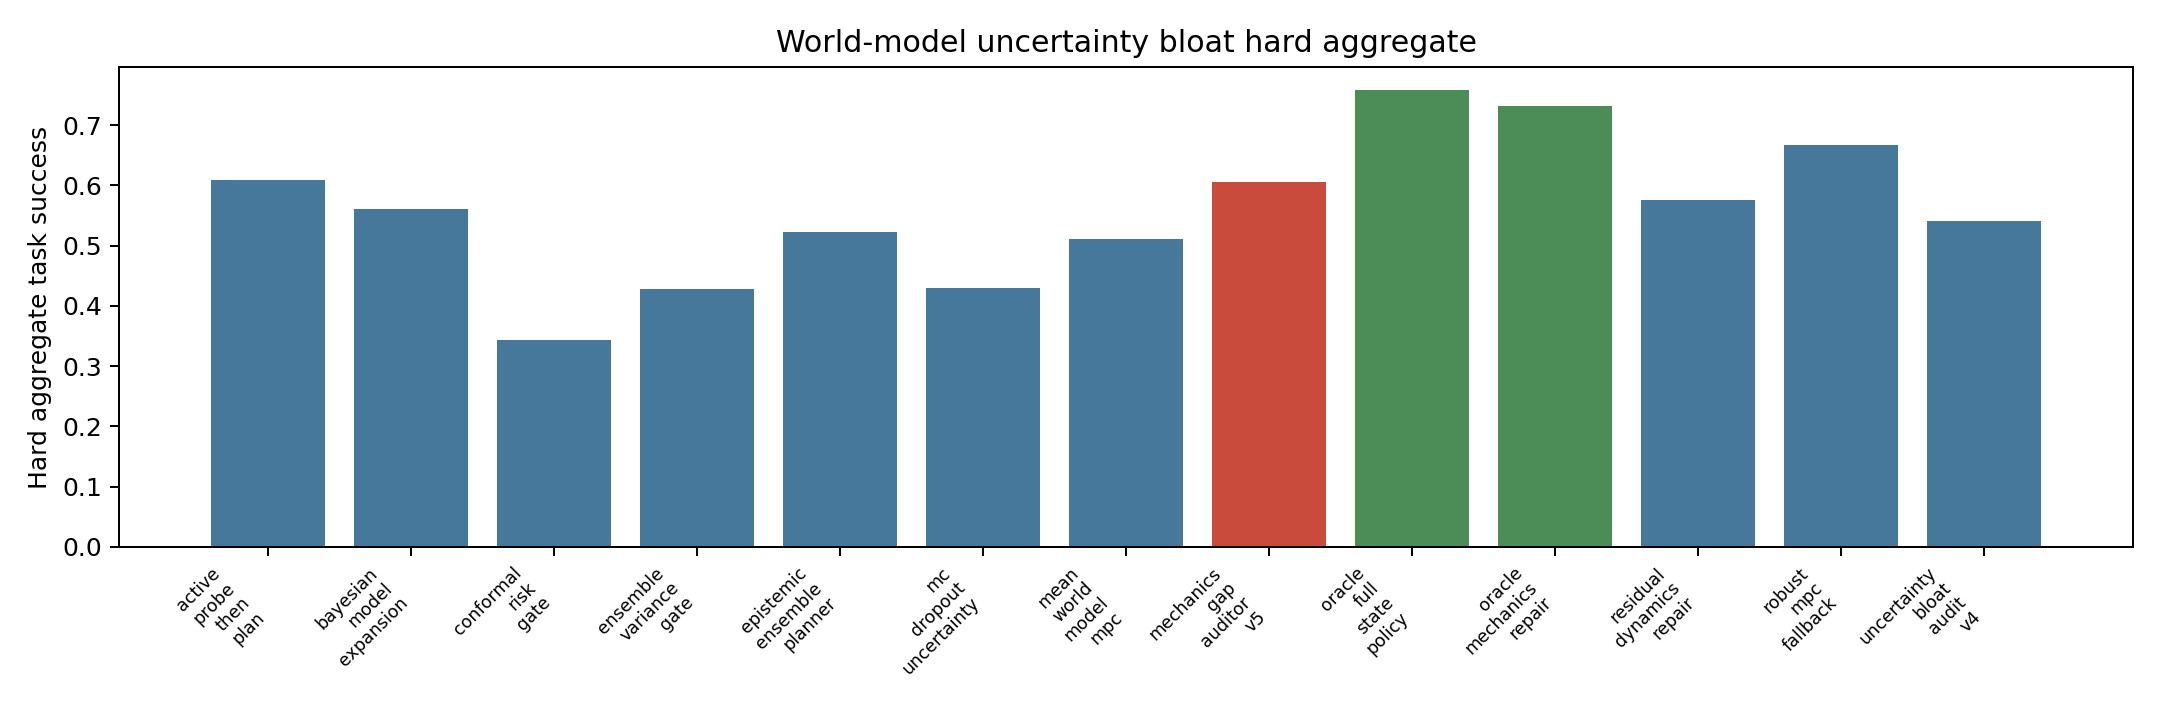
\includegraphics[width=0.95\linewidth]{uncertainty_bloat_hard_success_v5.png}\caption{Hard-aggregate task success. Robust MPC remains the strongest non-oracle success/utility reference.}\label{fig:hard-success}\end{figure}

\begin{figure}[t]\centering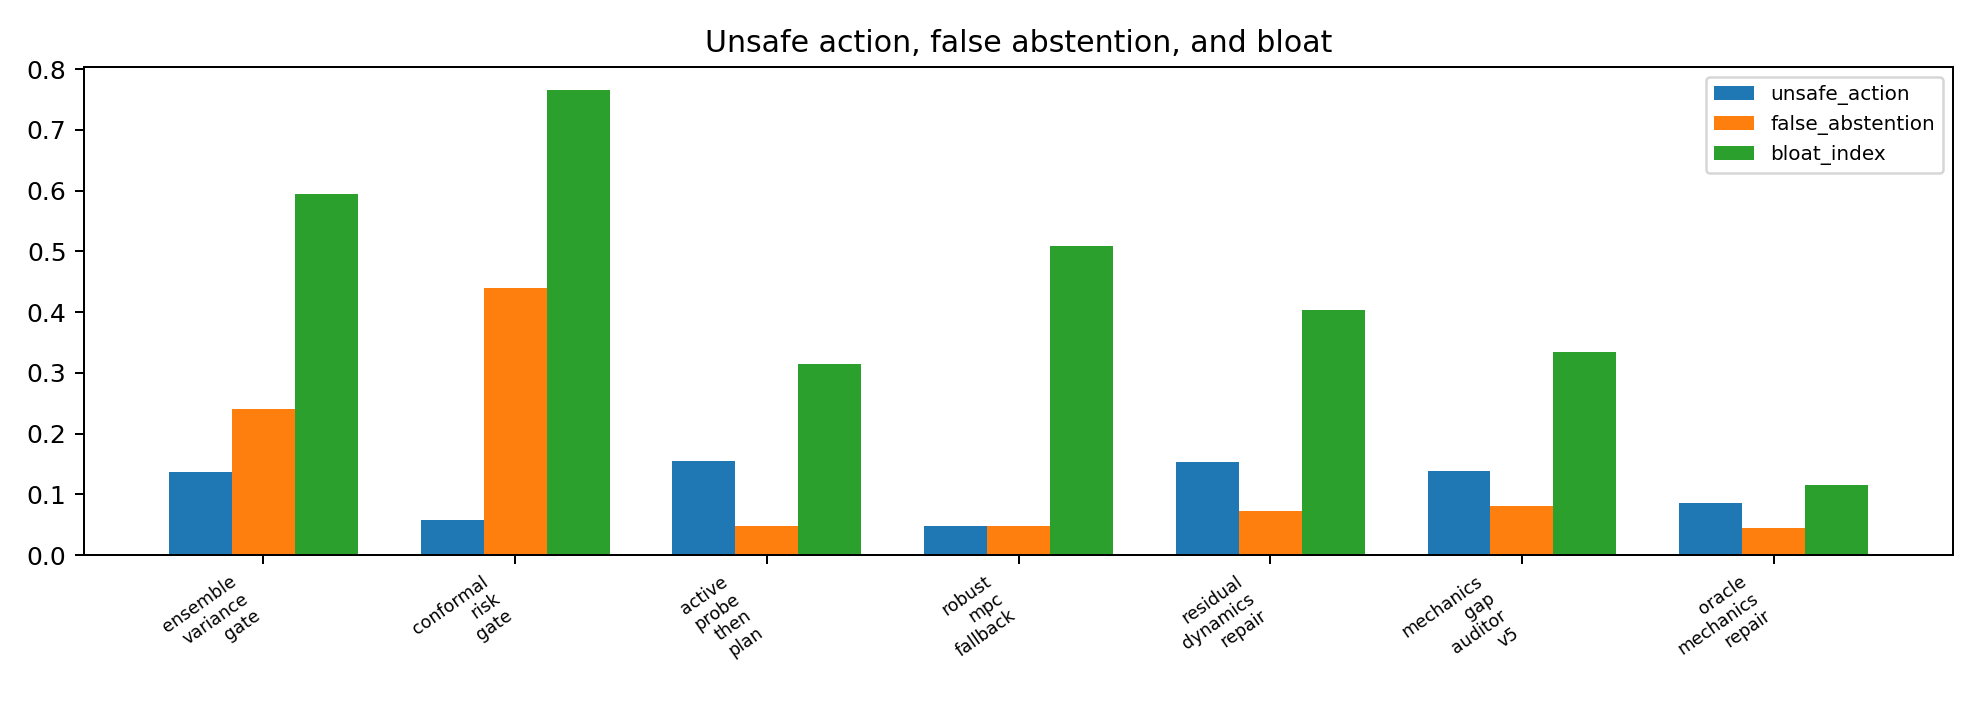
\includegraphics[width=0.95\linewidth]{uncertainty_bloat_failures_v5.png}\caption{Unsafe action, false abstention, and bloat. The v5 method improves some diagnostics but not enough to satisfy the safety gate.}\label{fig:failures}\end{figure}

\section{Split-Level Evidence}

The split-level table prevents the paper from hiding behind a single favorable split. The combined missing-mechanics regime remains the decisive test.

\begin{center}
\scriptsize
\begin{longtable}{p{0.16\linewidth}p{0.25\linewidth}rrrrr}
\caption{Split-level results for uncertainty, active-probe, robust, repair, v4, v5, and oracle methods.}\label{tab:split}\\
\toprule
Split & Method & Success & Mech. F1 & Unsafe & Bloat & Utility\\
\midrule
\endfirsthead
\caption[]{Split-level results for uncertainty, active-probe, robust, repair, v4, v5, and oracle methods. (continued)}\\
\toprule
Split & Method & Success & Mech. F1 & Unsafe & Bloat & Utility\\
\midrule
\endhead
Nominal & Ensemble variance & 0.531 $\pm$ 0.027 & 0.211 & 0.069 & 0.531 & 0.095\\
Nominal & Conformal gate & 0.439 $\pm$ 0.026 & 0.146 & 0.008 & 0.688 & -0.092\\
Nominal & Active probe & 0.730 $\pm$ 0.028 & 0.237 & 0.100 & 0.275 & 0.477\\
Nominal & Robust MPC & 0.812 $\pm$ 0.014 & 0.138 & 0.001 & 0.429 & 0.658\\
Nominal & Residual repair & 0.730 $\pm$ 0.024 & 0.244 & 0.081 & 0.350 & 0.472\\
Nominal & Bayesian expansion & 0.702 $\pm$ 0.014 & 0.226 & 0.067 & 0.372 & 0.436\\
Nominal & Bloat audit v4 & 0.678 $\pm$ 0.015 & 0.248 & 0.106 & 0.452 & 0.363\\
Nominal & Mechanics gap v5 & 0.723 $\pm$ 0.018 & 0.229 & 0.069 & 0.296 & 0.493\\
Nominal & Oracle repair & 0.769 $\pm$ 0.014 & 0.256 & 0.080 & 0.120 & 0.590\\
Friction/contact & Ensemble variance & 0.497 $\pm$ 0.035 & 0.346 & 0.088 & 0.566 & 0.015\\
Friction/contact & Conformal gate & 0.376 $\pm$ 0.019 & 0.251 & 0.041 & 0.731 & -0.249\\
Friction/contact & Active probe & 0.674 $\pm$ 0.013 & 0.517 & 0.116 & 0.290 & 0.381\\
Friction/contact & Robust MPC & 0.749 $\pm$ 0.016 & 0.182 & 0.022 & 0.472 & 0.543\\
Friction/contact & Residual repair & 0.637 $\pm$ 0.011 & 0.453 & 0.125 & 0.373 & 0.297\\
Friction/contact & Bayesian expansion & 0.623 $\pm$ 0.020 & 0.499 & 0.107 & 0.390 & 0.275\\
Friction/contact & Bloat audit v4 & 0.627 $\pm$ 0.025 & 0.415 & 0.129 & 0.481 & 0.250\\
Friction/contact & Mechanics gap v5 & 0.696 $\pm$ 0.023 & 0.516 & 0.093 & 0.309 & 0.422\\
Friction/contact & Oracle repair & 0.768 $\pm$ 0.014 & 0.602 & 0.071 & 0.110 & 0.585\\
Actuator sat. & Ensemble variance & 0.510 $\pm$ 0.020 & 0.359 & 0.088 & 0.572 & 0.038\\
Actuator sat. & Conformal gate & 0.403 $\pm$ 0.016 & 0.269 & 0.036 & 0.735 & -0.192\\
Actuator sat. & Active probe & 0.648 $\pm$ 0.023 & 0.517 & 0.142 & 0.296 & 0.324\\
Actuator sat. & Robust MPC & 0.727 $\pm$ 0.018 & 0.153 & 0.026 & 0.480 & 0.516\\
Actuator sat. & Residual repair & 0.643 $\pm$ 0.020 & 0.423 & 0.120 & 0.384 & 0.302\\
Actuator sat. & Bayesian expansion & 0.604 $\pm$ 0.018 & 0.500 & 0.114 & 0.397 & 0.243\\
Actuator sat. & Bloat audit v4 & 0.601 $\pm$ 0.015 & 0.431 & 0.137 & 0.489 & 0.207\\
Actuator sat. & Mechanics gap v5 & 0.685 $\pm$ 0.018 & 0.539 & 0.095 & 0.315 & 0.399\\
Actuator sat. & Oracle repair & 0.768 $\pm$ 0.018 & 0.622 & 0.069 & 0.110 & 0.591\\
Sensor dropout & Ensemble variance & 0.519 $\pm$ 0.015 & 0.311 & 0.085 & 0.581 & 0.038\\
Sensor dropout & Conformal gate & 0.392 $\pm$ 0.016 & 0.197 & 0.033 & 0.744 & -0.209\\
Sensor dropout & Active probe & 0.667 $\pm$ 0.015 & 0.474 & 0.135 & 0.310 & 0.345\\
Sensor dropout & Robust MPC & 0.733 $\pm$ 0.027 & 0.051 & 0.022 & 0.489 & 0.515\\
Sensor dropout & Residual repair & 0.634 $\pm$ 0.019 & 0.370 & 0.113 & 0.395 & 0.300\\
Sensor dropout & Bayesian expansion & 0.642 $\pm$ 0.027 & 0.462 & 0.102 & 0.409 & 0.291\\
Sensor dropout & Bloat audit v4 & 0.607 $\pm$ 0.022 & 0.339 & 0.139 & 0.500 & 0.213\\
Sensor dropout & Mechanics gap v5 & 0.656 $\pm$ 0.025 & 0.449 & 0.106 & 0.332 & 0.351\\
Sensor dropout & Oracle repair & 0.739 $\pm$ 0.027 & 0.554 & 0.082 & 0.133 & 0.537\\
Latency/hyst. & Ensemble variance & 0.482 $\pm$ 0.017 & 0.396 & 0.096 & 0.573 & -0.015\\
Latency/hyst. & Conformal gate & 0.367 $\pm$ 0.017 & 0.241 & 0.032 & 0.742 & -0.258\\
Latency/hyst. & Active probe & 0.662 $\pm$ 0.021 & 0.504 & 0.136 & 0.303 & 0.336\\
Latency/hyst. & Robust MPC & 0.736 $\pm$ 0.025 & 0.167 & 0.019 & 0.484 & 0.522\\
Latency/hyst. & Residual repair & 0.636 $\pm$ 0.024 & 0.433 & 0.127 & 0.384 & 0.290\\
Latency/hyst. & Bayesian expansion & 0.625 $\pm$ 0.008 & 0.471 & 0.102 & 0.404 & 0.278\\
Latency/hyst. & Bloat audit v4 & 0.602 $\pm$ 0.020 & 0.417 & 0.146 & 0.493 & 0.193\\
Latency/hyst. & Mechanics gap v5 & 0.663 $\pm$ 0.017 & 0.490 & 0.094 & 0.324 & 0.377\\
Latency/hyst. & Oracle repair & 0.752 $\pm$ 0.017 & 0.616 & 0.079 & 0.117 & 0.556\\
Latent fixture & Ensemble variance & 0.458 $\pm$ 0.021 & 0.401 & 0.118 & 0.579 & -0.064\\
Latent fixture & Conformal gate & 0.356 $\pm$ 0.019 & 0.246 & 0.047 & 0.750 & -0.280\\
Latent fixture & Active probe & 0.653 $\pm$ 0.016 & 0.534 & 0.140 & 0.304 & 0.317\\
Latent fixture & Robust MPC & 0.691 $\pm$ 0.024 & 0.136 & 0.034 & 0.493 & 0.454\\
Latent fixture & Residual repair & 0.607 $\pm$ 0.023 & 0.464 & 0.138 & 0.392 & 0.233\\
Latent fixture & Bayesian expansion & 0.596 $\pm$ 0.030 & 0.516 & 0.120 & 0.407 & 0.223\\
Latent fixture & Bloat audit v4 & 0.583 $\pm$ 0.031 & 0.437 & 0.148 & 0.499 & 0.167\\
Latent fixture & Mechanics gap v5 & 0.644 $\pm$ 0.026 & 0.558 & 0.124 & 0.324 & 0.305\\
Latent fixture & Oracle repair & 0.754 $\pm$ 0.020 & 0.683 & 0.081 & 0.112 & 0.556\\
Missing contact & Ensemble variance & 0.428 $\pm$ 0.022 & 0.422 & 0.130 & 0.591 & -0.132\\
Missing contact & Conformal gate & 0.357 $\pm$ 0.028 & 0.245 & 0.063 & 0.762 & -0.299\\
Missing contact & Active probe & 0.608 $\pm$ 0.019 & 0.575 & 0.152 & 0.313 & 0.245\\
Missing contact & Robust MPC & 0.669 $\pm$ 0.021 & 0.159 & 0.046 & 0.507 & 0.408\\
Missing contact & Residual repair & 0.582 $\pm$ 0.021 & 0.485 & 0.155 & 0.402 & 0.184\\
Missing contact & Bayesian expansion & 0.562 $\pm$ 0.029 & 0.551 & 0.133 & 0.416 & 0.150\\
Missing contact & Bloat audit v4 & 0.543 $\pm$ 0.031 & 0.460 & 0.163 & 0.507 & 0.092\\
Missing contact & Mechanics gap v5 & 0.624 $\pm$ 0.025 & 0.580 & 0.122 & 0.332 & 0.278\\
Missing contact & Oracle repair & 0.755 $\pm$ 0.021 & 0.722 & 0.075 & 0.112 & 0.562\\
Combined missing & Ensemble variance & 0.398 $\pm$ 0.021 & 0.393 & 0.164 & 0.614 & -0.227\\
Combined missing & Conformal gate & 0.318 $\pm$ 0.015 & 0.259 & 0.062 & 0.782 & -0.364\\
Combined missing & Active probe & 0.567 $\pm$ 0.024 & 0.599 & 0.174 & 0.327 & 0.163\\
Combined missing & Robust MPC & 0.641 $\pm$ 0.023 & 0.139 & 0.066 & 0.528 & 0.334\\
Combined missing & Residual repair & 0.537 $\pm$ 0.014 & 0.515 & 0.166 & 0.418 & 0.093\\
Combined missing & Bayesian expansion & 0.524 $\pm$ 0.021 & 0.575 & 0.143 & 0.430 & 0.079\\
Combined missing & Bloat audit v4 & 0.496 $\pm$ 0.021 & 0.450 & 0.190 & 0.527 & -0.010\\
Combined missing & Mechanics gap v5 & 0.551 $\pm$ 0.020 & 0.629 & 0.167 & 0.347 & 0.129\\
Combined missing & Oracle repair & 0.689 $\pm$ 0.017 & 0.775 & 0.100 & 0.121 & 0.442\\
\bottomrule
\end{longtable}
\normalsize
\end{center}

\section{Paired Comparisons}

Paired seed tests are harsher than independent means. V5 beats the old v4 audit on several diagnostic metrics, but it trails robust MPC on success and utility and has a positive unsafe-action difference.

\begin{center}
\scriptsize
\begin{longtable}{p{0.29\linewidth}p{0.21\linewidth}rrrr}
\caption{Paired seed-level differences for mechanics gap v5 minus selected references on the hard aggregate.}\label{tab:paired}\\
\toprule
Reference & Metric & Mean diff & CI95 & Lower95 & Upper95\\
\midrule
\endfirsthead
\caption[]{Paired seed-level differences for mechanics gap v5 minus selected references on the hard aggregate. (continued)}\\
\toprule
Reference & Metric & Mean diff & CI95 & Lower95 & Upper95\\
\midrule
\endhead
Robust MPC & Success & -0.061 & 0.017 & -0.077 & -0.044\\
Robust MPC & Mech. F1 & 0.444 & 0.022 & 0.423 & 0.466\\
Robust MPC & Unsafe & 0.089 & 0.014 & 0.075 & 0.103\\
Robust MPC & Bloat & -0.175 & 0.002 & -0.177 & -0.173\\
Robust MPC & Utility & -0.162 & 0.032 & -0.193 & -0.130\\
Active probe & Success & -0.003 & 0.018 & -0.021 & 0.015\\
Active probe & Mech. F1 & 0.019 & 0.023 & -0.004 & 0.042\\
Active probe & Unsafe & -0.018 & 0.016 & -0.033 & -0.002\\
Active probe & Bloat & 0.020 & 0.002 & 0.017 & 0.022\\
Active probe & Utility & -0.005 & 0.040 & -0.045 & 0.035\\
Bloat audit v4 & Success & 0.066 & 0.023 & 0.043 & 0.088\\
Bloat audit v4 & Mech. F1 & 0.140 & 0.019 & 0.121 & 0.159\\
Bloat audit v4 & Unsafe & -0.029 & 0.017 & -0.046 & -0.012\\
Bloat audit v4 & Bloat & -0.177 & 0.002 & -0.179 & -0.174\\
Bloat audit v4 & Utility & 0.154 & 0.047 & 0.107 & 0.201\\
\bottomrule
\end{longtable}
\normalsize
\end{center}

\section{Mechanism Ablations}

The ablation story is mixed. Removing repair memory improves combined-split success and utility in this synthetic audit, while removing false-abstention penalty lowers unsafe actions. That means the mechanism is not yet clean enough for an ICLR-main claim.

\begin{center}
\scriptsize
\begin{longtable}{p{0.16\linewidth}p{0.27\linewidth}rrrrr}
\caption{Mechanism ablations. The full system had to beat every removal on robust utility and avoid success/safety reversals.}\label{tab:ablation}\\
\toprule
Split & Ablation & Success & Mech. F1 & Unsafe & Bloat & Utility\\
\midrule
\endfirsthead
\caption[]{Mechanism ablations. The full system had to beat every removal on robust utility and avoid success/safety reversals. (continued)}\\
\toprule
Split & Ablation & Success & Mech. F1 & Unsafe & Bloat & Utility\\
\midrule
\endhead
Missing contact & Full mechanics gap v5 & 0.607 $\pm$ 0.030 & 0.600 & 0.121 & 0.333 & 0.250\\
Missing contact & - mechanism classifier & 0.595 $\pm$ 0.024 & 0.448 & 0.132 & 0.478 & 0.201\\
Missing contact & - bloat index & 0.502 $\pm$ 0.022 & 0.552 & 0.133 & 0.611 & -0.033\\
Missing contact & - active probe value & 0.573 $\pm$ 0.021 & 0.542 & 0.124 & 0.350 & 0.210\\
Missing contact & - repair memory & 0.601 $\pm$ 0.025 & 0.557 & 0.132 & 0.371 & 0.235\\
Missing contact & - abstention penalty & 0.546 $\pm$ 0.018 & 0.593 & 0.095 & 0.344 & 0.138\\
Missing contact & - calibrated risk & 0.599 $\pm$ 0.021 & 0.573 & 0.152 & 0.394 & 0.196\\
Missing contact & Variance-only bloat & 0.460 $\pm$ 0.028 & 0.493 & 0.096 & 0.613 & -0.063\\
Missing contact & Abstain-only & 0.290 $\pm$ 0.025 & 0.162 & 0.046 & 0.765 & -0.413\\
Missing contact & Probe no memory & 0.592 $\pm$ 0.026 & 0.586 & 0.133 & 0.419 & 0.208\\
Combined missing & Full mechanics gap v5 & 0.556 $\pm$ 0.017 & 0.620 & 0.152 & 0.350 & 0.148\\
Combined missing & - mechanism classifier & 0.533 $\pm$ 0.026 & 0.407 & 0.166 & 0.502 & 0.070\\
Combined missing & - bloat index & 0.485 $\pm$ 0.023 & 0.586 & 0.148 & 0.622 & -0.065\\
Combined missing & - active probe value & 0.546 $\pm$ 0.015 & 0.552 & 0.159 & 0.363 & 0.134\\
Combined missing & - repair memory & 0.574 $\pm$ 0.021 & 0.606 & 0.148 & 0.383 & 0.179\\
Combined missing & - abstention penalty & 0.526 $\pm$ 0.030 & 0.624 & 0.101 & 0.357 & 0.107\\
Combined missing & - calibrated risk & 0.554 $\pm$ 0.035 & 0.619 & 0.177 & 0.408 & 0.103\\
Combined missing & Variance-only bloat & 0.418 $\pm$ 0.034 & 0.523 & 0.153 & 0.628 & -0.191\\
Combined missing & Abstain-only & 0.258 $\pm$ 0.027 & 0.154 & 0.052 & 0.787 & -0.487\\
Combined missing & Probe no memory & 0.559 $\pm$ 0.025 & 0.598 & 0.158 & 0.437 & 0.127\\
\bottomrule
\end{longtable}
\normalsize
\end{center}

\begin{figure}[t]\centering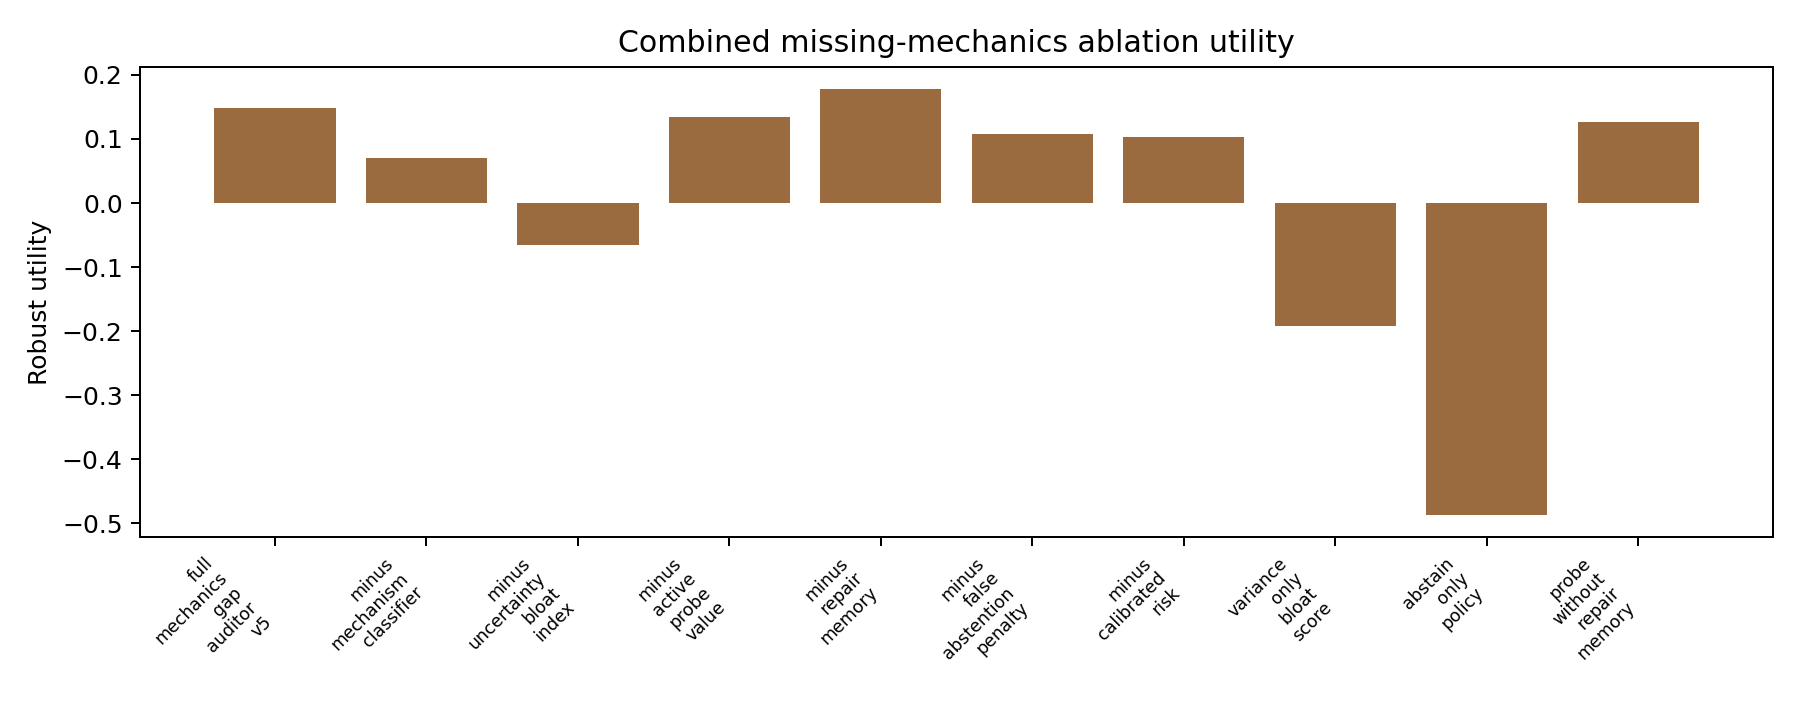
\includegraphics[width=0.95\linewidth]{uncertainty_bloat_ablation_v5.png}\caption{Combined missing-mechanics ablation utility. The full mechanism fails the frozen ablation gate.}\label{fig:ablation}\end{figure}

\section{Stress Testing}

The stress gate passes because v5 is not Pareto dominated at maximum combined stress. That is not enough to rescue the paper because the main, mechanism, fixed-risk, and scope gates fail.

\begin{figure}[t]\centering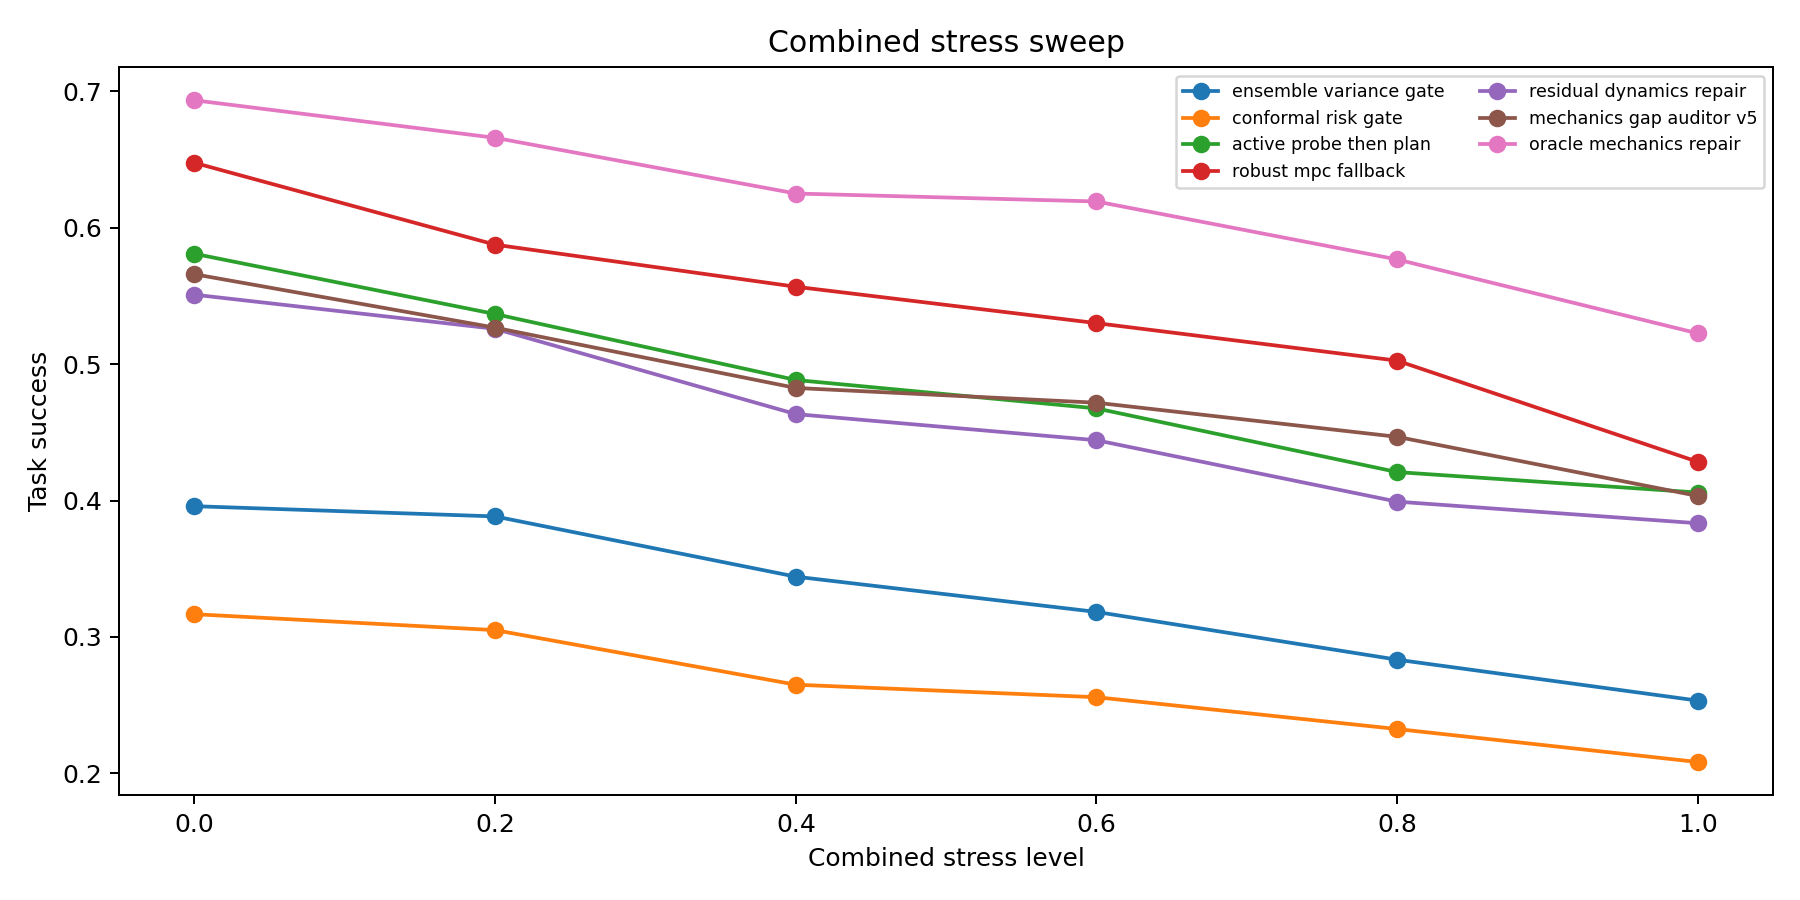
\includegraphics[width=0.95\linewidth]{uncertainty_bloat_stress_sweep_v5.png}\caption{Task success under combined stress.}\label{fig:stress}\end{figure}

\begin{center}
\scriptsize
\begin{longtable}{p{0.18\linewidth}rp{0.23\linewidth}rrrrr}
\caption{Full stress sweep over all six axes and six levels. The table is complete so favorable plots cannot hide unfavorable regimes.}\label{tab:stress}\\
\toprule
Axis & Level & Method & Succ. & Mech. F1 & Unsafe & Bloat & Utility\\
\midrule
\endfirsthead
\caption[]{Full stress sweep over all six axes and six levels. The table is complete so favorable plots cannot hide unfavorable regimes. (continued)}\\
\toprule
Axis & Level & Method & Succ. & Mech. F1 & Unsafe & Bloat & Utility\\
\midrule
\endhead
contact friction shift & 0.0 & Ensemble variance & 0.403 & 0.397 & 0.151 & 0.612 & -0.194\\
contact friction shift & 0.0 & Conformal gate & 0.304 & 0.206 & 0.057 & 0.788 & -0.398\\
contact friction shift & 0.0 & Active probe & 0.554 & 0.599 & 0.179 & 0.328 & 0.136\\
contact friction shift & 0.0 & Robust MPC & 0.617 & 0.145 & 0.062 & 0.527 & 0.316\\
contact friction shift & 0.0 & Residual repair & 0.550 & 0.519 & 0.180 & 0.414 & 0.104\\
contact friction shift & 0.0 & Mechanics gap v5 & 0.554 & 0.585 & 0.168 & 0.352 & 0.132\\
contact friction shift & 0.0 & Oracle repair & 0.682 & 0.773 & 0.102 & 0.122 & 0.429\\
contact friction shift & 0.2 & Ensemble variance & 0.396 & 0.427 & 0.137 & 0.609 & -0.197\\
contact friction shift & 0.2 & Conformal gate & 0.314 & 0.265 & 0.071 & 0.781 & -0.383\\
contact friction shift & 0.2 & Active probe & 0.559 & 0.589 & 0.203 & 0.330 & 0.105\\
contact friction shift & 0.2 & Robust MPC & 0.636 & 0.143 & 0.074 & 0.526 & 0.323\\
contact friction shift & 0.2 & Residual repair & 0.547 & 0.510 & 0.150 & 0.412 & 0.130\\
contact friction shift & 0.2 & Mechanics gap v5 & 0.569 & 0.602 & 0.157 & 0.348 & 0.169\\
contact friction shift & 0.2 & Oracle repair & 0.651 & 0.749 & 0.110 & 0.125 & 0.385\\
contact friction shift & 0.4 & Ensemble variance & 0.384 & 0.420 & 0.145 & 0.612 & -0.227\\
contact friction shift & 0.4 & Conformal gate & 0.302 & 0.267 & 0.075 & 0.782 & -0.404\\
contact friction shift & 0.4 & Active probe & 0.561 & 0.600 & 0.177 & 0.326 & 0.142\\
contact friction shift & 0.4 & Robust MPC & 0.598 & 0.176 & 0.088 & 0.526 & 0.261\\
contact friction shift & 0.4 & Residual repair & 0.530 & 0.508 & 0.172 & 0.416 & 0.071\\
contact friction shift & 0.4 & Mechanics gap v5 & 0.566 & 0.606 & 0.170 & 0.347 & 0.146\\
contact friction shift & 0.4 & Oracle repair & 0.674 & 0.770 & 0.093 & 0.120 & 0.437\\
contact friction shift & 0.6 & Ensemble variance & 0.372 & 0.437 & 0.164 & 0.606 & -0.251\\
contact friction shift & 0.6 & Conformal gate & 0.278 & 0.288 & 0.066 & 0.777 & -0.428\\
contact friction shift & 0.6 & Active probe & 0.571 & 0.622 & 0.195 & 0.321 & 0.129\\
contact friction shift & 0.6 & Robust MPC & 0.608 & 0.147 & 0.095 & 0.523 & 0.261\\
contact friction shift & 0.6 & Residual repair & 0.520 & 0.483 & 0.187 & 0.416 & 0.063\\
contact friction shift & 0.6 & Mechanics gap v5 & 0.565 & 0.581 & 0.150 & 0.349 & 0.163\\
contact friction shift & 0.6 & Oracle repair & 0.661 & 0.762 & 0.104 & 0.123 & 0.403\\
contact friction shift & 0.8 & Ensemble variance & 0.368 & 0.442 & 0.179 & 0.607 & -0.251\\
contact friction shift & 0.8 & Conformal gate & 0.274 & 0.282 & 0.095 & 0.778 & -0.445\\
contact friction shift & 0.8 & Active probe & 0.519 & 0.608 & 0.193 & 0.331 & 0.072\\
contact friction shift & 0.8 & Robust MPC & 0.550 & 0.165 & 0.092 & 0.530 & 0.193\\
contact friction shift & 0.8 & Residual repair & 0.512 & 0.542 & 0.193 & 0.412 & 0.034\\
contact friction shift & 0.8 & Mechanics gap v5 & 0.497 & 0.631 & 0.186 & 0.344 & 0.044\\
contact friction shift & 0.8 & Oracle repair & 0.676 & 0.788 & 0.107 & 0.119 & 0.418\\
contact friction shift & 1.0 & Ensemble variance & 0.367 & 0.401 & 0.159 & 0.611 & -0.236\\
contact friction shift & 1.0 & Conformal gate & 0.267 & 0.299 & 0.098 & 0.775 & -0.438\\
contact friction shift & 1.0 & Active probe & 0.491 & 0.635 & 0.233 & 0.321 & 0.001\\
contact friction shift & 1.0 & Robust MPC & 0.569 & 0.173 & 0.098 & 0.529 & 0.208\\
contact friction shift & 1.0 & Residual repair & 0.486 & 0.519 & 0.201 & 0.416 & -0.005\\
contact friction shift & 1.0 & Mechanics gap v5 & 0.515 & 0.646 & 0.177 & 0.342 & 0.076\\
contact friction shift & 1.0 & Oracle repair & 0.642 & 0.788 & 0.118 & 0.117 & 0.369\\
actuator saturation & 0.0 & Ensemble variance & 0.393 & 0.410 & 0.135 & 0.615 & -0.204\\
actuator saturation & 0.0 & Conformal gate & 0.312 & 0.231 & 0.065 & 0.788 & -0.395\\
actuator saturation & 0.0 & Active probe & 0.586 & 0.611 & 0.170 & 0.326 & 0.180\\
actuator saturation & 0.0 & Robust MPC & 0.622 & 0.185 & 0.070 & 0.529 & 0.303\\
actuator saturation & 0.0 & Residual repair & 0.554 & 0.523 & 0.167 & 0.417 & 0.119\\
actuator saturation & 0.0 & Mechanics gap v5 & 0.571 & 0.633 & 0.143 & 0.346 & 0.187\\
actuator saturation & 0.0 & Oracle repair & 0.692 & 0.775 & 0.105 & 0.122 & 0.441\\
actuator saturation & 0.2 & Ensemble variance & 0.412 & 0.431 & 0.141 & 0.608 & -0.165\\
actuator saturation & 0.2 & Conformal gate & 0.308 & 0.282 & 0.077 & 0.781 & -0.394\\
actuator saturation & 0.2 & Active probe & 0.547 & 0.618 & 0.180 & 0.328 & 0.125\\
actuator saturation & 0.2 & Robust MPC & 0.587 & 0.143 & 0.075 & 0.530 & 0.255\\
actuator saturation & 0.2 & Residual repair & 0.542 & 0.507 & 0.156 & 0.417 & 0.112\\
actuator saturation & 0.2 & Mechanics gap v5 & 0.562 & 0.622 & 0.166 & 0.344 & 0.155\\
actuator saturation & 0.2 & Oracle repair & 0.672 & 0.790 & 0.109 & 0.120 & 0.416\\
actuator saturation & 0.4 & Ensemble variance & 0.398 & 0.376 & 0.157 & 0.615 & -0.223\\
actuator saturation & 0.4 & Conformal gate & 0.308 & 0.301 & 0.066 & 0.780 & -0.394\\
actuator saturation & 0.4 & Active probe & 0.560 & 0.603 & 0.172 & 0.329 & 0.138\\
actuator saturation & 0.4 & Robust MPC & 0.623 & 0.160 & 0.077 & 0.529 & 0.291\\
actuator saturation & 0.4 & Residual repair & 0.526 & 0.513 & 0.156 & 0.419 & 0.098\\
actuator saturation & 0.4 & Mechanics gap v5 & 0.542 & 0.623 & 0.169 & 0.345 & 0.123\\
actuator saturation & 0.4 & Oracle repair & 0.667 & 0.776 & 0.110 & 0.119 & 0.406\\
actuator saturation & 0.6 & Ensemble variance & 0.363 & 0.441 & 0.144 & 0.609 & -0.251\\
actuator saturation & 0.6 & Conformal gate & 0.313 & 0.283 & 0.077 & 0.777 & -0.368\\
actuator saturation & 0.6 & Active probe & 0.532 & 0.595 & 0.225 & 0.327 & 0.051\\
actuator saturation & 0.6 & Robust MPC & 0.621 & 0.174 & 0.080 & 0.526 & 0.290\\
actuator saturation & 0.6 & Residual repair & 0.506 & 0.494 & 0.178 & 0.420 & 0.048\\
actuator saturation & 0.6 & Mechanics gap v5 & 0.533 & 0.602 & 0.183 & 0.350 & 0.078\\
actuator saturation & 0.6 & Oracle repair & 0.650 & 0.777 & 0.112 & 0.120 & 0.395\\
actuator saturation & 0.8 & Ensemble variance & 0.396 & 0.459 & 0.161 & 0.607 & -0.209\\
actuator saturation & 0.8 & Conformal gate & 0.260 & 0.271 & 0.081 & 0.783 & -0.456\\
actuator saturation & 0.8 & Active probe & 0.527 & 0.642 & 0.223 & 0.324 & 0.050\\
actuator saturation & 0.8 & Robust MPC & 0.591 & 0.170 & 0.092 & 0.528 & 0.241\\
actuator saturation & 0.8 & Residual repair & 0.504 & 0.505 & 0.189 & 0.420 & 0.032\\
actuator saturation & 0.8 & Mechanics gap v5 & 0.542 & 0.630 & 0.168 & 0.345 & 0.115\\
actuator saturation & 0.8 & Oracle repair & 0.657 & 0.780 & 0.117 & 0.119 & 0.390\\
actuator saturation & 1.0 & Ensemble variance & 0.378 & 0.424 & 0.164 & 0.610 & -0.239\\
actuator saturation & 1.0 & Conformal gate & 0.285 & 0.258 & 0.101 & 0.778 & -0.429\\
actuator saturation & 1.0 & Active probe & 0.505 & 0.615 & 0.207 & 0.329 & 0.036\\
actuator saturation & 1.0 & Robust MPC & 0.568 & 0.165 & 0.100 & 0.528 & 0.201\\
actuator saturation & 1.0 & Residual repair & 0.497 & 0.541 & 0.191 & 0.411 & 0.020\\
actuator saturation & 1.0 & Mechanics gap v5 & 0.506 & 0.639 & 0.176 & 0.343 & 0.063\\
actuator saturation & 1.0 & Oracle repair & 0.618 & 0.771 & 0.123 & 0.121 & 0.340\\
sensor dropout & 0.0 & Ensemble variance & 0.400 & 0.396 & 0.157 & 0.610 & -0.195\\
sensor dropout & 0.0 & Conformal gate & 0.297 & 0.263 & 0.073 & 0.784 & -0.420\\
sensor dropout & 0.0 & Active probe & 0.562 & 0.579 & 0.204 & 0.330 & 0.122\\
sensor dropout & 0.0 & Robust MPC & 0.637 & 0.135 & 0.062 & 0.528 & 0.339\\
sensor dropout & 0.0 & Residual repair & 0.512 & 0.506 & 0.173 & 0.417 & 0.065\\
sensor dropout & 0.0 & Mechanics gap v5 & 0.581 & 0.629 & 0.136 & 0.344 & 0.204\\
sensor dropout & 0.0 & Oracle repair & 0.695 & 0.764 & 0.096 & 0.123 & 0.458\\
sensor dropout & 0.2 & Ensemble variance & 0.382 & 0.398 & 0.151 & 0.619 & -0.227\\
sensor dropout & 0.2 & Conformal gate & 0.296 & 0.214 & 0.064 & 0.793 & -0.412\\
sensor dropout & 0.2 & Active probe & 0.564 & 0.561 & 0.175 & 0.340 & 0.147\\
sensor dropout & 0.2 & Robust MPC & 0.627 & 0.121 & 0.068 & 0.538 & 0.307\\
sensor dropout & 0.2 & Residual repair & 0.539 & 0.503 & 0.168 & 0.425 & 0.094\\
sensor dropout & 0.2 & Mechanics gap v5 & 0.561 & 0.583 & 0.149 & 0.356 & 0.164\\
sensor dropout & 0.2 & Oracle repair & 0.704 & 0.766 & 0.106 & 0.128 & 0.461\\
sensor dropout & 0.4 & Ensemble variance & 0.382 & 0.376 & 0.150 & 0.629 & -0.231\\
sensor dropout & 0.4 & Conformal gate & 0.312 & 0.219 & 0.052 & 0.800 & -0.381\\
sensor dropout & 0.4 & Active probe & 0.542 & 0.584 & 0.197 & 0.343 & 0.101\\
sensor dropout & 0.4 & Robust MPC & 0.608 & 0.080 & 0.072 & 0.546 & 0.280\\
sensor dropout & 0.4 & Residual repair & 0.524 & 0.460 & 0.163 & 0.438 & 0.077\\
sensor dropout & 0.4 & Mechanics gap v5 & 0.559 & 0.563 & 0.156 & 0.369 & 0.147\\
sensor dropout & 0.4 & Oracle repair & 0.661 & 0.761 & 0.113 & 0.141 & 0.394\\
sensor dropout & 0.6 & Ensemble variance & 0.406 & 0.362 & 0.142 & 0.635 & -0.195\\
sensor dropout & 0.6 & Conformal gate & 0.304 & 0.197 & 0.079 & 0.804 & -0.410\\
sensor dropout & 0.6 & Active probe & 0.534 & 0.583 & 0.184 & 0.352 & 0.090\\
sensor dropout & 0.6 & Robust MPC & 0.583 & 0.066 & 0.087 & 0.552 & 0.234\\
sensor dropout & 0.6 & Residual repair & 0.534 & 0.458 & 0.156 & 0.444 & 0.091\\
sensor dropout & 0.6 & Mechanics gap v5 & 0.537 & 0.570 & 0.145 & 0.374 & 0.128\\
sensor dropout & 0.6 & Oracle repair & 0.639 & 0.746 & 0.119 & 0.151 & 0.346\\
sensor dropout & 0.8 & Ensemble variance & 0.369 & 0.344 & 0.150 & 0.644 & -0.243\\
sensor dropout & 0.8 & Conformal gate & 0.284 & 0.162 & 0.079 & 0.814 & -0.434\\
sensor dropout & 0.8 & Active probe & 0.514 & 0.545 & 0.206 & 0.368 & 0.039\\
sensor dropout & 0.8 & Robust MPC & 0.597 & 0.031 & 0.075 & 0.561 & 0.260\\
sensor dropout & 0.8 & Residual repair & 0.515 & 0.441 & 0.177 & 0.451 & 0.045\\
sensor dropout & 0.8 & Mechanics gap v5 & 0.539 & 0.568 & 0.142 & 0.385 & 0.132\\
sensor dropout & 0.8 & Oracle repair & 0.625 & 0.746 & 0.121 & 0.159 & 0.334\\
sensor dropout & 1.0 & Ensemble variance & 0.371 & 0.328 & 0.161 & 0.652 & -0.256\\
sensor dropout & 1.0 & Conformal gate & 0.289 & 0.153 & 0.076 & 0.817 & -0.408\\
sensor dropout & 1.0 & Active probe & 0.523 & 0.573 & 0.197 & 0.369 & 0.058\\
sensor dropout & 1.0 & Robust MPC & 0.610 & 0.007 & 0.084 & 0.567 & 0.269\\
sensor dropout & 1.0 & Residual repair & 0.495 & 0.425 & 0.182 & 0.461 & 0.021\\
sensor dropout & 1.0 & Mechanics gap v5 & 0.514 & 0.549 & 0.187 & 0.392 & 0.056\\
sensor dropout & 1.0 & Oracle repair & 0.626 & 0.749 & 0.107 & 0.165 & 0.357\\
latency hysteresis & 0.0 & Ensemble variance & 0.420 & 0.384 & 0.142 & 0.610 & -0.166\\
latency hysteresis & 0.0 & Conformal gate & 0.310 & 0.301 & 0.073 & 0.778 & -0.391\\
latency hysteresis & 0.0 & Active probe & 0.573 & 0.596 & 0.186 & 0.327 & 0.150\\
latency hysteresis & 0.0 & Robust MPC & 0.619 & 0.157 & 0.062 & 0.527 & 0.317\\
latency hysteresis & 0.0 & Residual repair & 0.532 & 0.477 & 0.179 & 0.419 & 0.074\\
latency hysteresis & 0.0 & Mechanics gap v5 & 0.574 & 0.614 & 0.147 & 0.344 & 0.182\\
latency hysteresis & 0.0 & Oracle repair & 0.683 & 0.758 & 0.113 & 0.126 & 0.422\\
latency hysteresis & 0.2 & Ensemble variance & 0.422 & 0.394 & 0.114 & 0.611 & -0.143\\
latency hysteresis & 0.2 & Conformal gate & 0.315 & 0.282 & 0.059 & 0.778 & -0.374\\
latency hysteresis & 0.2 & Active probe & 0.562 & 0.573 & 0.202 & 0.329 & 0.119\\
latency hysteresis & 0.2 & Robust MPC & 0.617 & 0.150 & 0.075 & 0.526 & 0.295\\
latency hysteresis & 0.2 & Residual repair & 0.538 & 0.492 & 0.159 & 0.417 & 0.114\\
latency hysteresis & 0.2 & Mechanics gap v5 & 0.573 & 0.588 & 0.139 & 0.347 & 0.192\\
latency hysteresis & 0.2 & Oracle repair & 0.661 & 0.769 & 0.099 & 0.123 & 0.405\\
latency hysteresis & 0.4 & Ensemble variance & 0.392 & 0.417 & 0.148 & 0.612 & -0.211\\
latency hysteresis & 0.4 & Conformal gate & 0.314 & 0.240 & 0.062 & 0.786 & -0.377\\
latency hysteresis & 0.4 & Active probe & 0.544 & 0.600 & 0.182 & 0.329 & 0.118\\
latency hysteresis & 0.4 & Robust MPC & 0.614 & 0.148 & 0.072 & 0.529 & 0.291\\
latency hysteresis & 0.4 & Residual repair & 0.512 & 0.508 & 0.188 & 0.417 & 0.050\\
latency hysteresis & 0.4 & Mechanics gap v5 & 0.549 & 0.620 & 0.147 & 0.347 & 0.143\\
latency hysteresis & 0.4 & Oracle repair & 0.667 & 0.765 & 0.110 & 0.123 & 0.410\\
latency hysteresis & 0.6 & Ensemble variance & 0.375 & 0.415 & 0.158 & 0.609 & -0.254\\
latency hysteresis & 0.6 & Conformal gate & 0.300 & 0.241 & 0.075 & 0.782 & -0.406\\
latency hysteresis & 0.6 & Active probe & 0.551 & 0.592 & 0.196 & 0.327 & 0.116\\
latency hysteresis & 0.6 & Robust MPC & 0.603 & 0.160 & 0.068 & 0.525 & 0.285\\
latency hysteresis & 0.6 & Residual repair & 0.520 & 0.487 & 0.172 & 0.416 & 0.068\\
latency hysteresis & 0.6 & Mechanics gap v5 & 0.564 & 0.597 & 0.172 & 0.345 & 0.138\\
latency hysteresis & 0.6 & Oracle repair & 0.644 & 0.735 & 0.128 & 0.131 & 0.359\\
latency hysteresis & 0.8 & Ensemble variance & 0.394 & 0.453 & 0.159 & 0.608 & -0.219\\
latency hysteresis & 0.8 & Conformal gate & 0.292 & 0.283 & 0.090 & 0.780 & -0.419\\
latency hysteresis & 0.8 & Active probe & 0.524 & 0.646 & 0.202 & 0.324 & 0.070\\
latency hysteresis & 0.8 & Robust MPC & 0.574 & 0.157 & 0.086 & 0.531 & 0.225\\
latency hysteresis & 0.8 & Residual repair & 0.487 & 0.518 & 0.184 & 0.418 & 0.006\\
latency hysteresis & 0.8 & Mechanics gap v5 & 0.527 & 0.620 & 0.175 & 0.349 & 0.078\\
latency hysteresis & 0.8 & Oracle repair & 0.664 & 0.779 & 0.122 & 0.120 & 0.384\\
latency hysteresis & 1.0 & Ensemble variance & 0.398 & 0.390 & 0.144 & 0.613 & -0.196\\
latency hysteresis & 1.0 & Conformal gate & 0.283 & 0.295 & 0.084 & 0.777 & -0.415\\
latency hysteresis & 1.0 & Active probe & 0.512 & 0.615 & 0.208 & 0.323 & 0.053\\
latency hysteresis & 1.0 & Robust MPC & 0.562 & 0.165 & 0.095 & 0.527 & 0.204\\
latency hysteresis & 1.0 & Residual repair & 0.510 & 0.513 & 0.183 & 0.418 & 0.046\\
latency hysteresis & 1.0 & Mechanics gap v5 & 0.521 & 0.627 & 0.179 & 0.344 & 0.086\\
latency hysteresis & 1.0 & Oracle repair & 0.640 & 0.774 & 0.128 & 0.120 & 0.356\\
hidden fixture rate & 0.0 & Ensemble variance & 0.396 & 0.429 & 0.140 & 0.612 & -0.203\\
hidden fixture rate & 0.0 & Conformal gate & 0.332 & 0.259 & 0.056 & 0.783 & -0.339\\
hidden fixture rate & 0.0 & Active probe & 0.573 & 0.577 & 0.195 & 0.330 & 0.142\\
hidden fixture rate & 0.0 & Robust MPC & 0.620 & 0.135 & 0.077 & 0.527 & 0.305\\
hidden fixture rate & 0.0 & Residual repair & 0.517 & 0.537 & 0.163 & 0.416 & 0.082\\
hidden fixture rate & 0.0 & Mechanics gap v5 & 0.572 & 0.617 & 0.140 & 0.345 & 0.178\\
hidden fixture rate & 0.0 & Oracle repair & 0.693 & 0.777 & 0.095 & 0.120 & 0.456\\
hidden fixture rate & 0.2 & Ensemble variance & 0.366 & 0.412 & 0.157 & 0.618 & -0.262\\
hidden fixture rate & 0.2 & Conformal gate & 0.325 & 0.258 & 0.076 & 0.785 & -0.365\\
hidden fixture rate & 0.2 & Active probe & 0.561 & 0.613 & 0.183 & 0.329 & 0.134\\
hidden fixture rate & 0.2 & Robust MPC & 0.608 & 0.158 & 0.074 & 0.535 & 0.278\\
hidden fixture rate & 0.2 & Residual repair & 0.532 & 0.506 & 0.173 & 0.424 & 0.076\\
hidden fixture rate & 0.2 & Mechanics gap v5 & 0.536 & 0.629 & 0.164 & 0.350 & 0.116\\
hidden fixture rate & 0.2 & Oracle repair & 0.682 & 0.797 & 0.100 & 0.114 & 0.442\\
hidden fixture rate & 0.4 & Ensemble variance & 0.337 & 0.411 & 0.169 & 0.628 & -0.324\\
hidden fixture rate & 0.4 & Conformal gate & 0.279 & 0.258 & 0.086 & 0.798 & -0.458\\
hidden fixture rate & 0.4 & Active probe & 0.562 & 0.640 & 0.192 & 0.332 & 0.130\\
hidden fixture rate & 0.4 & Robust MPC & 0.579 & 0.165 & 0.092 & 0.545 & 0.219\\
hidden fixture rate & 0.4 & Residual repair & 0.512 & 0.518 & 0.194 & 0.427 & 0.034\\
hidden fixture rate & 0.4 & Mechanics gap v5 & 0.550 & 0.673 & 0.164 & 0.352 & 0.116\\
hidden fixture rate & 0.4 & Oracle repair & 0.711 & 0.840 & 0.111 & 0.109 & 0.468\\
hidden fixture rate & 0.6 & Ensemble variance & 0.346 & 0.417 & 0.177 & 0.628 & -0.310\\
hidden fixture rate & 0.6 & Conformal gate & 0.272 & 0.265 & 0.097 & 0.803 & -0.468\\
hidden fixture rate & 0.6 & Active probe & 0.502 & 0.659 & 0.234 & 0.331 & 0.006\\
hidden fixture rate & 0.6 & Robust MPC & 0.586 & 0.156 & 0.078 & 0.549 & 0.249\\
hidden fixture rate & 0.6 & Residual repair & 0.487 & 0.519 & 0.203 & 0.435 & -0.022\\
hidden fixture rate & 0.6 & Mechanics gap v5 & 0.532 & 0.665 & 0.177 & 0.352 & 0.085\\
hidden fixture rate & 0.6 & Oracle repair & 0.655 & 0.858 & 0.132 & 0.113 & 0.364\\
hidden fixture rate & 0.8 & Ensemble variance & 0.318 & 0.429 & 0.196 & 0.635 & -0.370\\
hidden fixture rate & 0.8 & Conformal gate & 0.248 & 0.280 & 0.092 & 0.809 & -0.507\\
hidden fixture rate & 0.8 & Active probe & 0.508 & 0.673 & 0.224 & 0.334 & 0.023\\
hidden fixture rate & 0.8 & Robust MPC & 0.515 & 0.153 & 0.122 & 0.559 & 0.105\\
hidden fixture rate & 0.8 & Residual repair & 0.502 & 0.532 & 0.219 & 0.433 & -0.006\\
hidden fixture rate & 0.8 & Mechanics gap v5 & 0.495 & 0.677 & 0.201 & 0.355 & 0.022\\
hidden fixture rate & 0.8 & Oracle repair & 0.661 & 0.885 & 0.126 & 0.108 & 0.382\\
hidden fixture rate & 1.0 & Ensemble variance & 0.319 & 0.441 & 0.200 & 0.638 & -0.360\\
hidden fixture rate & 1.0 & Conformal gate & 0.233 & 0.296 & 0.117 & 0.811 & -0.524\\
hidden fixture rate & 1.0 & Active probe & 0.453 & 0.693 & 0.259 & 0.339 & -0.089\\
hidden fixture rate & 1.0 & Robust MPC & 0.501 & 0.164 & 0.144 & 0.568 & 0.057\\
hidden fixture rate & 1.0 & Residual repair & 0.441 & 0.573 & 0.234 & 0.431 & -0.096\\
hidden fixture rate & 1.0 & Mechanics gap v5 & 0.482 & 0.709 & 0.229 & 0.351 & -0.023\\
hidden fixture rate & 1.0 & Oracle repair & 0.645 & 0.914 & 0.134 & 0.104 & 0.355\\
combined & 0.0 & Ensemble variance & 0.396 & 0.370 & 0.133 & 0.616 & -0.203\\
combined & 0.0 & Conformal gate & 0.317 & 0.266 & 0.072 & 0.781 & -0.389\\
combined & 0.0 & Active probe & 0.581 & 0.607 & 0.186 & 0.327 & 0.158\\
combined & 0.0 & Robust MPC & 0.647 & 0.138 & 0.069 & 0.526 & 0.342\\
combined & 0.0 & Residual repair & 0.551 & 0.525 & 0.165 & 0.414 & 0.118\\
combined & 0.0 & Mechanics gap v5 & 0.566 & 0.618 & 0.158 & 0.345 & 0.159\\
combined & 0.0 & Oracle repair & 0.693 & 0.763 & 0.089 & 0.123 & 0.467\\
combined & 0.2 & Ensemble variance & 0.388 & 0.429 & 0.153 & 0.619 & -0.235\\
combined & 0.2 & Conformal gate & 0.305 & 0.287 & 0.072 & 0.790 & -0.408\\
combined & 0.2 & Active probe & 0.537 & 0.611 & 0.196 & 0.334 & 0.098\\
combined & 0.2 & Robust MPC & 0.588 & 0.164 & 0.078 & 0.538 & 0.248\\
combined & 0.2 & Residual repair & 0.526 & 0.480 & 0.174 & 0.426 & 0.072\\
combined & 0.2 & Mechanics gap v5 & 0.527 & 0.623 & 0.170 & 0.355 & 0.086\\
combined & 0.2 & Oracle repair & 0.666 & 0.775 & 0.113 & 0.127 & 0.404\\
combined & 0.4 & Ensemble variance & 0.344 & 0.423 & 0.176 & 0.625 & -0.294\\
combined & 0.4 & Conformal gate & 0.265 & 0.279 & 0.089 & 0.793 & -0.438\\
combined & 0.4 & Active probe & 0.488 & 0.626 & 0.207 & 0.345 & 0.014\\
combined & 0.4 & Robust MPC & 0.557 & 0.121 & 0.100 & 0.550 & 0.187\\
combined & 0.4 & Residual repair & 0.463 & 0.515 & 0.217 & 0.433 & -0.057\\
combined & 0.4 & Mechanics gap v5 & 0.482 & 0.624 & 0.193 & 0.363 & 0.010\\
combined & 0.4 & Oracle repair & 0.625 & 0.814 & 0.139 & 0.128 & 0.318\\
combined & 0.6 & Ensemble variance & 0.318 & 0.420 & 0.190 & 0.631 & -0.318\\
combined & 0.6 & Conformal gate & 0.256 & 0.275 & 0.114 & 0.797 & -0.440\\
combined & 0.6 & Active probe & 0.468 & 0.623 & 0.229 & 0.351 & -0.034\\
combined & 0.6 & Robust MPC & 0.530 & 0.150 & 0.120 & 0.556 & 0.131\\
combined & 0.6 & Residual repair & 0.444 & 0.501 & 0.227 & 0.443 & -0.096\\
combined & 0.6 & Mechanics gap v5 & 0.472 & 0.639 & 0.197 & 0.369 & -0.003\\
combined & 0.6 & Oracle repair & 0.619 & 0.829 & 0.130 & 0.131 & 0.326\\
combined & 0.8 & Ensemble variance & 0.283 & 0.443 & 0.211 & 0.635 & -0.366\\
combined & 0.8 & Conformal gate & 0.233 & 0.292 & 0.113 & 0.795 & -0.405\\
combined & 0.8 & Active probe & 0.421 & 0.658 & 0.253 & 0.352 & -0.113\\
combined & 0.8 & Robust MPC & 0.502 & 0.140 & 0.142 & 0.568 & 0.070\\
combined & 0.8 & Residual repair & 0.399 & 0.548 & 0.227 & 0.447 & -0.136\\
combined & 0.8 & Mechanics gap v5 & 0.447 & 0.651 & 0.236 & 0.371 & -0.076\\
combined & 0.8 & Oracle repair & 0.577 & 0.857 & 0.159 & 0.131 & 0.254\\
combined & 1.0 & Ensemble variance & 0.253 & 0.460 & 0.223 & 0.638 & -0.400\\
combined & 1.0 & Conformal gate & 0.208 & 0.295 & 0.131 & 0.801 & -0.435\\
combined & 1.0 & Active probe & 0.406 & 0.651 & 0.267 & 0.360 & -0.144\\
combined & 1.0 & Robust MPC & 0.428 & 0.131 & 0.156 & 0.578 & -0.027\\
combined & 1.0 & Residual repair & 0.383 & 0.558 & 0.247 & 0.450 & -0.177\\
combined & 1.0 & Mechanics gap v5 & 0.403 & 0.683 & 0.259 & 0.378 & -0.145\\
combined & 1.0 & Oracle repair & 0.522 & 0.875 & 0.173 & 0.134 & 0.175\\
\bottomrule
\end{longtable}
\normalsize
\end{center}

\section{Fixed-Risk Deployment}

The fixed-risk gate is the cleanest deployment failure. At budget 0.05, all non-oracle methods have zero accepted coverage on the hard fixed-risk splits. A reviewer should treat this as a blocker because the system cannot claim safe operation by refusing every hard episode.

\begin{figure}[t]\centering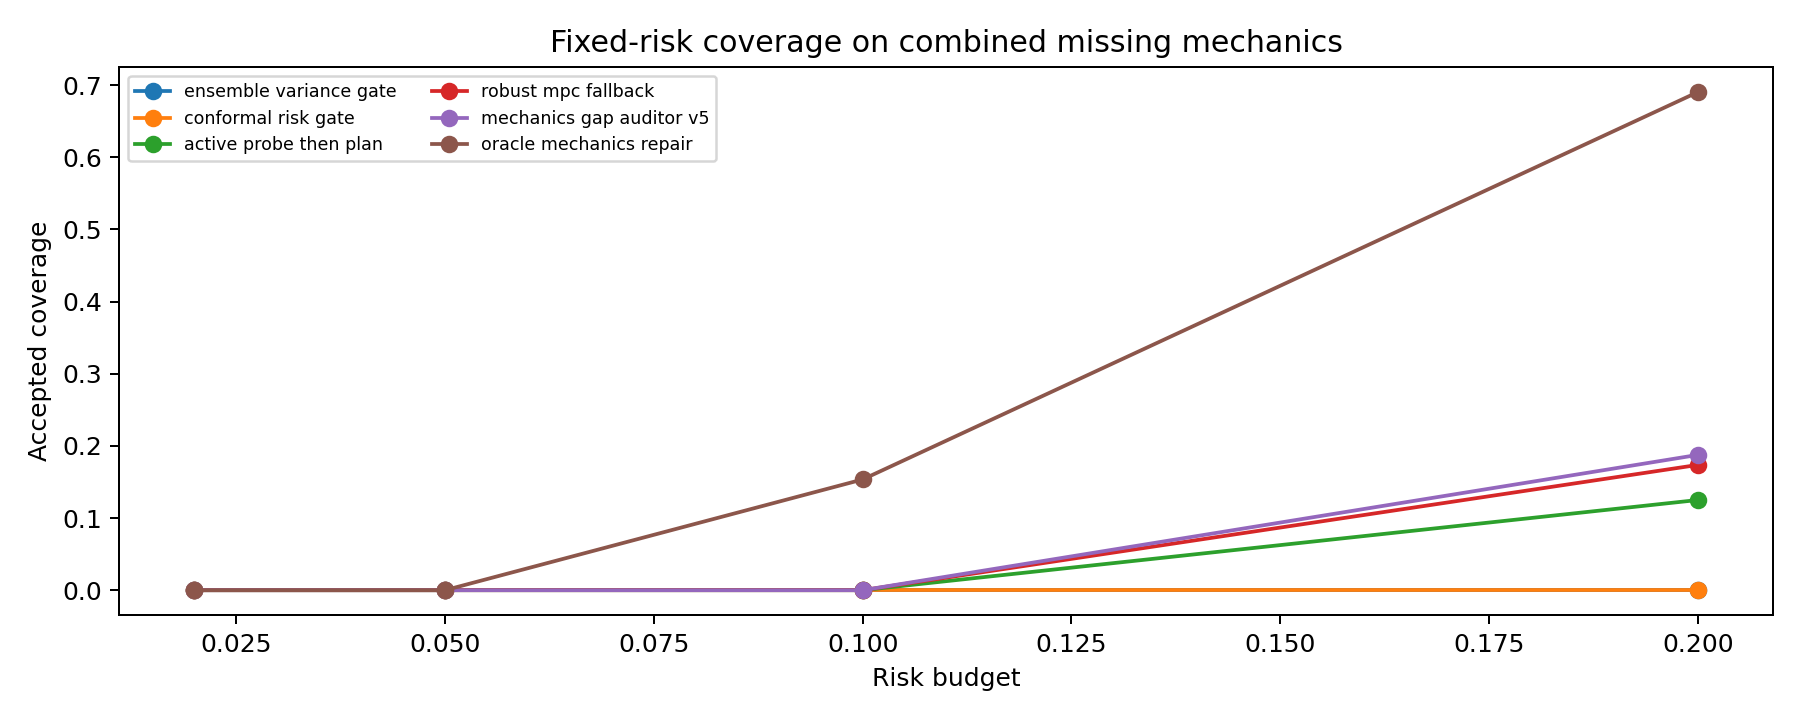
\includegraphics[width=0.95\linewidth]{uncertainty_bloat_fixed_risk_v5.png}\caption{Fixed-risk coverage on combined missing mechanics. Strict coverage collapses.}\label{fig:fixed}\end{figure}

\begin{center}
\scriptsize
\begin{longtable}{p{0.16\linewidth}rp{0.23\linewidth}rrrrr}
\caption{Fixed-risk deployment results. A low-risk policy must have nonzero coverage, not just low accepted failure rates after rejecting hard cases.}\label{tab:fixed}\\
\toprule
Split & Budget & Method & Cover. & Succ. & Unsafe & Bloat & Mean risk\\
\midrule
\endfirsthead
\caption[]{Fixed-risk deployment results. A low-risk policy must have nonzero coverage, not just low accepted failure rates after rejecting hard cases. (continued)}\\
\toprule
Split & Budget & Method & Cover. & Succ. & Unsafe & Bloat & Mean risk\\
\midrule
\endhead
Missing contact & 0.02 & Ensemble variance & 0.000 & 0.000 & 0.000 & 0.000 & 0.349\\
Missing contact & 0.02 & Conformal gate & 0.000 & 0.000 & 0.000 & 0.000 & 0.352\\
Missing contact & 0.02 & Active probe & 0.000 & 0.000 & 0.000 & 0.000 & 0.261\\
Missing contact & 0.02 & Robust MPC & 0.000 & 0.000 & 0.000 & 0.000 & 0.239\\
Missing contact & 0.02 & Mechanics gap v5 & 0.000 & 0.000 & 0.000 & 0.000 & 0.249\\
Missing contact & 0.02 & Oracle repair & 0.000 & 0.000 & 0.000 & 0.000 & 0.156\\
Missing contact & 0.05 & Ensemble variance & 0.000 & 0.000 & 0.000 & 0.000 & 0.350\\
Missing contact & 0.05 & Conformal gate & 0.000 & 0.000 & 0.000 & 0.000 & 0.353\\
Missing contact & 0.05 & Active probe & 0.000 & 0.000 & 0.000 & 0.000 & 0.262\\
Missing contact & 0.05 & Robust MPC & 0.000 & 0.000 & 0.000 & 0.000 & 0.239\\
Missing contact & 0.05 & Mechanics gap v5 & 0.000 & 0.000 & 0.000 & 0.000 & 0.248\\
Missing contact & 0.05 & Oracle repair & 0.001 & 0.100 & 0.000 & 0.000 & 0.162\\
Missing contact & 0.10 & Ensemble variance & 0.000 & 0.000 & 0.000 & 0.000 & 0.348\\
Missing contact & 0.10 & Conformal gate & 0.000 & 0.000 & 0.000 & 0.000 & 0.352\\
Missing contact & 0.10 & Active probe & 0.001 & 0.100 & 0.000 & 0.012 & 0.262\\
Missing contact & 0.10 & Robust MPC & 0.000 & 0.000 & 0.000 & 0.000 & 0.239\\
Missing contact & 0.10 & Mechanics gap v5 & 0.002 & 0.200 & 0.000 & 0.030 & 0.247\\
Missing contact & 0.10 & Oracle repair & 0.208 & 0.957 & 0.000 & 0.012 & 0.160\\
Missing contact & 0.20 & Ensemble variance & 0.002 & 0.200 & 0.000 & 0.073 & 0.349\\
Missing contact & 0.20 & Conformal gate & 0.001 & 0.100 & 0.000 & 0.048 & 0.353\\
Missing contact & 0.20 & Active probe & 0.160 & 0.834 & 0.067 & 0.209 & 0.261\\
Missing contact & 0.20 & Robust MPC & 0.258 & 0.830 & 0.003 & 0.413 & 0.240\\
Missing contact & 0.20 & Mechanics gap v5 & 0.243 & 0.849 & 0.038 & 0.252 & 0.248\\
Missing contact & 0.20 & Oracle repair & 0.756 & 0.818 & 0.041 & 0.090 & 0.158\\
Combined missing & 0.02 & Ensemble variance & 0.000 & 0.000 & 0.000 & 0.000 & 0.366\\
Combined missing & 0.02 & Conformal gate & 0.000 & 0.000 & 0.000 & 0.000 & 0.373\\
Combined missing & 0.02 & Active probe & 0.000 & 0.000 & 0.000 & 0.000 & 0.279\\
Combined missing & 0.02 & Robust MPC & 0.000 & 0.000 & 0.000 & 0.000 & 0.256\\
Combined missing & 0.02 & Mechanics gap v5 & 0.000 & 0.000 & 0.000 & 0.000 & 0.264\\
Combined missing & 0.02 & Oracle repair & 0.000 & 0.000 & 0.000 & 0.000 & 0.173\\
Combined missing & 0.05 & Ensemble variance & 0.000 & 0.000 & 0.000 & 0.000 & 0.368\\
Combined missing & 0.05 & Conformal gate & 0.000 & 0.000 & 0.000 & 0.000 & 0.373\\
Combined missing & 0.05 & Active probe & 0.000 & 0.000 & 0.000 & 0.000 & 0.277\\
Combined missing & 0.05 & Robust MPC & 0.000 & 0.000 & 0.000 & 0.000 & 0.256\\
Combined missing & 0.05 & Mechanics gap v5 & 0.000 & 0.000 & 0.000 & 0.000 & 0.263\\
Combined missing & 0.05 & Oracle repair & 0.000 & 0.000 & 0.000 & 0.000 & 0.175\\
Combined missing & 0.10 & Ensemble variance & 0.000 & 0.000 & 0.000 & 0.000 & 0.368\\
Combined missing & 0.10 & Conformal gate & 0.000 & 0.000 & 0.000 & 0.000 & 0.371\\
Combined missing & 0.10 & Active probe & 0.000 & 0.000 & 0.000 & 0.000 & 0.280\\
Combined missing & 0.10 & Robust MPC & 0.000 & 0.000 & 0.000 & 0.000 & 0.256\\
Combined missing & 0.10 & Mechanics gap v5 & 0.000 & 0.000 & 0.000 & 0.000 & 0.267\\
Combined missing & 0.10 & Oracle repair & 0.153 & 0.895 & 0.018 & 0.017 & 0.168\\
Combined missing & 0.20 & Ensemble variance & 0.000 & 0.000 & 0.000 & 0.000 & 0.367\\
Combined missing & 0.20 & Conformal gate & 0.000 & 0.000 & 0.000 & 0.000 & 0.373\\
Combined missing & 0.20 & Active probe & 0.125 & 0.873 & 0.051 & 0.201 & 0.280\\
Combined missing & 0.20 & Robust MPC & 0.174 & 0.828 & 0.003 & 0.423 & 0.256\\
Combined missing & 0.20 & Mechanics gap v5 & 0.188 & 0.835 & 0.039 & 0.253 & 0.268\\
Combined missing & 0.20 & Oracle repair & 0.690 & 0.822 & 0.050 & 0.091 & 0.171\\
\bottomrule
\end{longtable}
\normalsize
\end{center}

\begin{center}
\scriptsize
\begin{longtable}{p{0.14\linewidth}rp{0.22\linewidth}p{0.18\linewidth}rrr}
\caption{Fixed-risk paired differences for v5 minus references at the deployment budgets emphasized in the frozen plan.}\label{tab:fixedpairs}\\
\toprule
Split & Budget & Reference & Metric & Mean diff & Lower95 & Upper95\\
\midrule
\endfirsthead
\caption[]{Fixed-risk paired differences for v5 minus references at the deployment budgets emphasized in the frozen plan. (continued)}\\
\toprule
Split & Budget & Reference & Metric & Mean diff & Lower95 & Upper95\\
\midrule
\endhead
Missing contact & 0.05 & Ensemble variance & Coverage & 0.000 & 0.000 & 0.000\\
Missing contact & 0.05 & Ensemble variance & Acc. succ. & 0.000 & 0.000 & 0.000\\
Missing contact & 0.05 & Ensemble variance & Acc. unsafe & 0.000 & 0.000 & 0.000\\
Missing contact & 0.05 & Ensemble variance & Acc. bloat & 0.000 & 0.000 & 0.000\\
Missing contact & 0.05 & Ensemble variance & Acc. utility & 0.000 & 0.000 & 0.000\\
Missing contact & 0.05 & Conformal gate & Coverage & 0.000 & 0.000 & 0.000\\
Missing contact & 0.05 & Conformal gate & Acc. succ. & 0.000 & 0.000 & 0.000\\
Missing contact & 0.05 & Conformal gate & Acc. unsafe & 0.000 & 0.000 & 0.000\\
Missing contact & 0.05 & Conformal gate & Acc. bloat & 0.000 & 0.000 & 0.000\\
Missing contact & 0.05 & Conformal gate & Acc. utility & 0.000 & 0.000 & 0.000\\
Missing contact & 0.05 & Active probe & Coverage & 0.000 & 0.000 & 0.000\\
Missing contact & 0.05 & Active probe & Acc. succ. & 0.000 & 0.000 & 0.000\\
Missing contact & 0.05 & Active probe & Acc. unsafe & 0.000 & 0.000 & 0.000\\
Missing contact & 0.05 & Active probe & Acc. bloat & 0.000 & 0.000 & 0.000\\
Missing contact & 0.05 & Active probe & Acc. utility & 0.000 & 0.000 & 0.000\\
Missing contact & 0.05 & Robust MPC & Coverage & 0.000 & 0.000 & 0.000\\
Missing contact & 0.05 & Robust MPC & Acc. succ. & 0.000 & 0.000 & 0.000\\
Missing contact & 0.05 & Robust MPC & Acc. unsafe & 0.000 & 0.000 & 0.000\\
Missing contact & 0.05 & Robust MPC & Acc. bloat & 0.000 & 0.000 & 0.000\\
Missing contact & 0.05 & Robust MPC & Acc. utility & 0.000 & 0.000 & 0.000\\
Missing contact & 0.05 & Oracle repair & Coverage & -0.001 & -0.002 & 0.001\\
Missing contact & 0.05 & Oracle repair & Acc. succ. & -0.100 & -0.296 & 0.096\\
Missing contact & 0.05 & Oracle repair & Acc. unsafe & 0.000 & 0.000 & 0.000\\
Missing contact & 0.05 & Oracle repair & Acc. bloat & 0.000 & 0.000 & 0.000\\
Missing contact & 0.05 & Oracle repair & Acc. utility & -0.097 & -0.288 & 0.093\\
Missing contact & 0.10 & Ensemble variance & Coverage & 0.002 & -0.001 & 0.005\\
Missing contact & 0.10 & Ensemble variance & Acc. succ. & 0.200 & -0.061 & 0.461\\
Missing contact & 0.10 & Ensemble variance & Acc. unsafe & 0.000 & 0.000 & 0.000\\
Missing contact & 0.10 & Ensemble variance & Acc. bloat & 0.030 & -0.009 & 0.070\\
Missing contact & 0.10 & Ensemble variance & Acc. utility & 0.182 & -0.056 & 0.419\\
Missing contact & 0.10 & Conformal gate & Coverage & 0.002 & -0.001 & 0.005\\
Missing contact & 0.10 & Conformal gate & Acc. succ. & 0.200 & -0.061 & 0.461\\
Missing contact & 0.10 & Conformal gate & Acc. unsafe & 0.000 & 0.000 & 0.000\\
Missing contact & 0.10 & Conformal gate & Acc. bloat & 0.030 & -0.009 & 0.070\\
Missing contact & 0.10 & Conformal gate & Acc. utility & 0.182 & -0.056 & 0.419\\
Missing contact & 0.10 & Active probe & Coverage & 0.001 & -0.002 & 0.005\\
Missing contact & 0.10 & Active probe & Acc. succ. & 0.100 & -0.252 & 0.452\\
Missing contact & 0.10 & Active probe & Acc. unsafe & 0.000 & 0.000 & 0.000\\
Missing contact & 0.10 & Active probe & Acc. bloat & 0.019 & -0.030 & 0.067\\
Missing contact & 0.10 & Active probe & Acc. utility & 0.088 & -0.236 & 0.412\\
Missing contact & 0.10 & Robust MPC & Coverage & 0.002 & -0.001 & 0.005\\
Missing contact & 0.10 & Robust MPC & Acc. succ. & 0.200 & -0.061 & 0.461\\
Missing contact & 0.10 & Robust MPC & Acc. unsafe & 0.000 & 0.000 & 0.000\\
Missing contact & 0.10 & Robust MPC & Acc. bloat & 0.030 & -0.009 & 0.070\\
Missing contact & 0.10 & Robust MPC & Acc. utility & 0.182 & -0.056 & 0.419\\
Missing contact & 0.10 & Oracle repair & Coverage & -0.206 & -0.228 & -0.183\\
Missing contact & 0.10 & Oracle repair & Acc. succ. & -0.757 & -1.016 & -0.498\\
Missing contact & 0.10 & Oracle repair & Acc. unsafe & 0.000 & 0.000 & 0.000\\
Missing contact & 0.10 & Oracle repair & Acc. bloat & 0.019 & -0.020 & 0.057\\
Missing contact & 0.10 & Oracle repair & Acc. utility & -0.737 & -0.972 & -0.502\\
Combined missing & 0.05 & Ensemble variance & Coverage & 0.000 & 0.000 & 0.000\\
Combined missing & 0.05 & Ensemble variance & Acc. succ. & 0.000 & 0.000 & 0.000\\
Combined missing & 0.05 & Ensemble variance & Acc. unsafe & 0.000 & 0.000 & 0.000\\
Combined missing & 0.05 & Ensemble variance & Acc. bloat & 0.000 & 0.000 & 0.000\\
Combined missing & 0.05 & Ensemble variance & Acc. utility & 0.000 & 0.000 & 0.000\\
Combined missing & 0.05 & Conformal gate & Coverage & 0.000 & 0.000 & 0.000\\
Combined missing & 0.05 & Conformal gate & Acc. succ. & 0.000 & 0.000 & 0.000\\
Combined missing & 0.05 & Conformal gate & Acc. unsafe & 0.000 & 0.000 & 0.000\\
Combined missing & 0.05 & Conformal gate & Acc. bloat & 0.000 & 0.000 & 0.000\\
Combined missing & 0.05 & Conformal gate & Acc. utility & 0.000 & 0.000 & 0.000\\
Combined missing & 0.05 & Active probe & Coverage & 0.000 & 0.000 & 0.000\\
Combined missing & 0.05 & Active probe & Acc. succ. & 0.000 & 0.000 & 0.000\\
Combined missing & 0.05 & Active probe & Acc. unsafe & 0.000 & 0.000 & 0.000\\
Combined missing & 0.05 & Active probe & Acc. bloat & 0.000 & 0.000 & 0.000\\
Combined missing & 0.05 & Active probe & Acc. utility & 0.000 & 0.000 & 0.000\\
Combined missing & 0.05 & Robust MPC & Coverage & 0.000 & 0.000 & 0.000\\
Combined missing & 0.05 & Robust MPC & Acc. succ. & 0.000 & 0.000 & 0.000\\
Combined missing & 0.05 & Robust MPC & Acc. unsafe & 0.000 & 0.000 & 0.000\\
Combined missing & 0.05 & Robust MPC & Acc. bloat & 0.000 & 0.000 & 0.000\\
Combined missing & 0.05 & Robust MPC & Acc. utility & 0.000 & 0.000 & 0.000\\
Combined missing & 0.05 & Oracle repair & Coverage & 0.000 & 0.000 & 0.000\\
Combined missing & 0.05 & Oracle repair & Acc. succ. & 0.000 & 0.000 & 0.000\\
Combined missing & 0.05 & Oracle repair & Acc. unsafe & 0.000 & 0.000 & 0.000\\
Combined missing & 0.05 & Oracle repair & Acc. bloat & 0.000 & 0.000 & 0.000\\
Combined missing & 0.05 & Oracle repair & Acc. utility & 0.000 & 0.000 & 0.000\\
Combined missing & 0.10 & Ensemble variance & Coverage & 0.000 & 0.000 & 0.000\\
Combined missing & 0.10 & Ensemble variance & Acc. succ. & 0.000 & 0.000 & 0.000\\
Combined missing & 0.10 & Ensemble variance & Acc. unsafe & 0.000 & 0.000 & 0.000\\
Combined missing & 0.10 & Ensemble variance & Acc. bloat & 0.000 & 0.000 & 0.000\\
Combined missing & 0.10 & Ensemble variance & Acc. utility & 0.000 & 0.000 & 0.000\\
Combined missing & 0.10 & Conformal gate & Coverage & 0.000 & 0.000 & 0.000\\
Combined missing & 0.10 & Conformal gate & Acc. succ. & 0.000 & 0.000 & 0.000\\
Combined missing & 0.10 & Conformal gate & Acc. unsafe & 0.000 & 0.000 & 0.000\\
Combined missing & 0.10 & Conformal gate & Acc. bloat & 0.000 & 0.000 & 0.000\\
Combined missing & 0.10 & Conformal gate & Acc. utility & 0.000 & 0.000 & 0.000\\
Combined missing & 0.10 & Active probe & Coverage & 0.000 & 0.000 & 0.000\\
Combined missing & 0.10 & Active probe & Acc. succ. & 0.000 & 0.000 & 0.000\\
Combined missing & 0.10 & Active probe & Acc. unsafe & 0.000 & 0.000 & 0.000\\
Combined missing & 0.10 & Active probe & Acc. bloat & 0.000 & 0.000 & 0.000\\
Combined missing & 0.10 & Active probe & Acc. utility & 0.000 & 0.000 & 0.000\\
Combined missing & 0.10 & Robust MPC & Coverage & 0.000 & 0.000 & 0.000\\
Combined missing & 0.10 & Robust MPC & Acc. succ. & 0.000 & 0.000 & 0.000\\
Combined missing & 0.10 & Robust MPC & Acc. unsafe & 0.000 & 0.000 & 0.000\\
Combined missing & 0.10 & Robust MPC & Acc. bloat & 0.000 & 0.000 & 0.000\\
Combined missing & 0.10 & Robust MPC & Acc. utility & 0.000 & 0.000 & 0.000\\
Combined missing & 0.10 & Oracle repair & Coverage & -0.153 & -0.169 & -0.138\\
Combined missing & 0.10 & Oracle repair & Acc. succ. & -0.895 & -0.949 & -0.840\\
Combined missing & 0.10 & Oracle repair & Acc. unsafe & -0.018 & -0.033 & -0.003\\
Combined missing & 0.10 & Oracle repair & Acc. bloat & -0.017 & -0.020 & -0.015\\
Combined missing & 0.10 & Oracle repair & Acc. utility & -0.833 & -0.901 & -0.766\\
\bottomrule
\end{longtable}
\normalsize
\end{center}

\section{Negative Cases}

The negative cases document exactly where uncertainty bloat, abstention, stale repair memory, and dropout false-gap diagnosis break the method.

\begin{center}
\scriptsize
\begin{longtable}{@{}p{0.16\linewidth}p{0.16\linewidth}p{0.36\linewidth}p{0.24\linewidth}@{}}
\caption{Predefined negative cases showing how uncertainty bloat, abstention, stale repair memory, and dropout false gaps fail.}\label{tab:negative}\\
\toprule
Case & Family & Observed failure & Terminal lesson\\
\midrule
\endfirsthead
\caption[]{Predefined negative cases showing how uncertainty bloat, abstention, stale repair memory, and dropout false gaps fail. (continued)}\\
\toprule
Case & Family & Observed failure & Terminal lesson\\
\midrule
\endhead
aleatoric noise as mechanics 0 & aleatoric noise as mechanics & variant 0: noise inflated as hidden contact gap & separate aleatoric noise from repairable structure\\
aleatoric noise as mechanics 1 & aleatoric noise as mechanics & variant 1: noise inflated as hidden contact gap & separate aleatoric noise from repairable structure\\
aleatoric noise as mechanics 2 & aleatoric noise as mechanics & variant 2: noise inflated as hidden contact gap & separate aleatoric noise from repairable structure\\
aleatoric noise as mechanics 3 & aleatoric noise as mechanics & variant 3: noise inflated as hidden contact gap & separate aleatoric noise from repairable structure\\
hidden contact mode bloat 0 & hidden contact mode bloat & variant 0: uncertainty gate abstains without repair & probe for contact mode rather than only abstaining\\
hidden contact mode bloat 1 & hidden contact mode bloat & variant 1: uncertainty gate abstains without repair & probe for contact mode rather than only abstaining\\
hidden contact mode bloat 2 & hidden contact mode bloat & variant 2: uncertainty gate abstains without repair & probe for contact mode rather than only abstaining\\
hidden contact mode bloat 3 & hidden contact mode bloat & variant 3: uncertainty gate abstains without repair & probe for contact mode rather than only abstaining\\
robust fallback overrepair 0 & robust fallback overrepair & variant 0: audit repairs a mechanism that robust MPC absorbs & repair must beat conservative control\\
robust fallback overrepair 1 & robust fallback overrepair & variant 1: audit repairs a mechanism that robust MPC absorbs & repair must beat conservative control\\
robust fallback overrepair 2 & robust fallback overrepair & variant 2: audit repairs a mechanism that robust MPC absorbs & repair must beat conservative control\\
robust fallback overrepair 3 & robust fallback overrepair & variant 3: audit repairs a mechanism that robust MPC absorbs & repair must beat conservative control\\
conformal zero coverage 0 & conformal zero coverage & variant 0: conformal gate rejects every hard episode & report coverage with accepted safety\\
conformal zero coverage 1 & conformal zero coverage & variant 1: conformal gate rejects every hard episode & report coverage with accepted safety\\
conformal zero coverage 2 & conformal zero coverage & variant 2: conformal gate rejects every hard episode & report coverage with accepted safety\\
conformal zero coverage 3 & conformal zero coverage & variant 3: conformal gate rejects every hard episode & report coverage with accepted safety\\
stale repair memory 0 & stale repair memory & variant 0: old fixture repair corrupts new task & mechanism memory needs expiry\\
stale repair memory 1 & stale repair memory & variant 1: old fixture repair corrupts new task & mechanism memory needs expiry\\
stale repair memory 2 & stale repair memory & variant 2: old fixture repair corrupts new task & mechanism memory needs expiry\\
stale repair memory 3 & stale repair memory & variant 3: old fixture repair corrupts new task & mechanism memory needs expiry\\
dropout false gap 0 & dropout false gap & variant 0: missing pixels become missing mechanics & diagnosis needs observation-quality state\\
dropout false gap 1 & dropout false gap & variant 1: missing pixels become missing mechanics & diagnosis needs observation-quality state\\
dropout false gap 2 & dropout false gap & variant 2: missing pixels become missing mechanics & diagnosis needs observation-quality state\\
dropout false gap 3 & dropout false gap & variant 3: missing pixels become missing mechanics & diagnosis needs observation-quality state\\
\bottomrule
\end{longtable}
\normalsize
\end{center}

\section{Prior Work Boundary}

The prior-work table is a novelty pressure device, not decoration. UQ, conformal safety, robust MPC, active perception, residual dynamics, and robot world-model work all threaten the claim \citep{pool88_01,pool88_02,pool88_03,pool88_04,pool88_05,pool88_06,pool88_07,pool88_08,pool88_09,pool88_10,pool88_11,pool88_12,pool88_13,pool88_14,pool88_15,pool88_16,pool88_17,pool88_18,pool88_19,pool88_20,pool88_21,pool88_22,pool88_23,pool88_24,pool88_25,pool88_26,pool88_27,pool88_28,pool88_29,pool88_30,pool88_31,pool88_32,pool88_33,pool88_34,pool88_35,pool88_36,pool88_37,pool88_38,pool88_39,pool88_40,pool88_41,pool88_42,pool88_43,pool88_44,pool88_45,pool88_46,pool88_47,pool88_48}. The current v5 evidence is not strong enough to overcome that boundary.

\begin{center}
\scriptsize
\begin{longtable}{p{0.12\linewidth}p{0.48\linewidth}p{0.14\linewidth}p{0.14\linewidth}r}
\caption{Closest local-pool references used to set the novelty boundary. The bright boxed citations jump to bibliography entries.}\label{tab:prior}\\
\toprule
Citation & Prior-work threat & Family & Role & Hostile\\
\midrule
\endfirsthead
\caption[]{Closest local-pool references used to set the novelty boundary. The bright boxed citations jump to bibliography entries. (continued)}\\
\toprule
Citation & Prior-work threat & Family & Role & Hostile\\
\midrule
\endhead
\citep{pool88_01} & An Investigation into Uncertainty Quantification of Shallow Foundation Failure Mechanisms in Horizontally Stratified Layered Soil Strata & failure & hostile & 27.000\\
\citep{pool88_02} & Mechanics of coordinative manipulation by multiple robotic mechanisms & openalex bulk robotics & concept & 20.771\\
\citep{pool88_03} & Action reliability analysis under random-interval hybrid uncertainty of chain conveyor based on adaptive intelligent extremum surrogate model & wam & concept & 19.999\\
\citep{pool88_04} & Deployment-Time Reliability of Learned Robot Policies & adaptation & concept & 21.550\\
\citep{pool88_05} & Reliability assessment of two-level balanced systems with common bus performance sharing subjected to epistemic uncertainty & ebm transformer & concept & 20.822\\
\citep{pool88_06} & Seven big ideas in robotics, and how to teach them & openalex bulk robotics & concept & 17.467\\
\citep{pool88_07} & Time-dependent reliability analysis of planar mechanisms considering truncated random variables and joint clearances & anti thesis & anti myopia & 20.320\\
\citep{pool88_08} & Reliability-based design optimization incorporating extended Optimal Uncertainty Quantification & anti thesis & anti myopia & 21.299\\
\citep{pool88_09} & Time-dependent kinematic reliability of motion mechanisms with dynamic factors & anti thesis & anti myopia & 20.242\\
\citep{pool88_10} & Optimization-Based Design for Specific Bistable Mechanics of Compliant Mechanisms & crossref bulk robotics & concept & 18.197\\
\citep{pool88_11} & Time-dependent reliability index for continuum structures against field uncertainty based on non-probabilistic bounded field model & anti thesis & anti myopia & 21.096\\
\citep{pool88_12} & Physics-integrated deep learning for uncertainty quantification and reliability estimation of nonlinear dynamical systems & anti thesis & anti myopia & 20.999\\
\citep{pool88_13} & Deep Reinforcement Learning for Fluid Mechanics: Control, Optimization, and Automation & ebm transformer & concept & 17.945\\
\citep{pool88_14} & Quantile-based sequential optimization and reliability assessment method under random and interval hybrid uncertainty & anti thesis & anti myopia & 20.896\\
\citep{pool88_15} & Toward Real-world BEV Perception: Depth Uncertainty Estimation via Gaussian Splatting & architecture & concept & 18.850\\
\citep{pool88_16} & Advanced sensor-based maintenance in real-world exemplary cases & ebm transformer & concept & 17.822\\
\citep{pool88_17} & ReconVLA: An Uncertainty-Guided and Failure-Aware Vision-Language-Action Framework for Robotic Control & anti thesis & anti myopia & 22.800\\
\citep{pool88_18} & Conversational Interfaces in IoT Ecosystems: Where We Are, What Is Still Missing & ebm transformer & concept & 17.799\\
\citep{pool88_19} & Data-driven polynomial chaos-interval metamodel for dynamics and reliability analysis under hybrid uncertainty & anti thesis & anti myopia & 20.773\\
\citep{pool88_20} & A comparison of deterministic, reliability-based and risk-based structural optimization under uncertainty & anti thesis & anti myopia & 20.678\\
\citep{pool88_21} & Minimally invasive laparoscopic and robot-assisted emergency treatment of strangulated giant hiatal hernias: report of five cases and literature review & openalex bulk robotics & concept & 16.646\\
\citep{pool88_22} & Towards Stronger Causal Claims in Management Research: Causal Triangulation Instead of Causal Identification & architecture & concept & 18.601\\
\citep{pool88_23} & Where Does It Belong? Autonomous Object Mapping in Open-World Settings & architecture & concept & 19.599\\
\citep{pool88_24} & A Bayesian approach to breaking things: efficiently predicting and repairing failure modes via sampling & failure & hostile & 21.450\\
\citep{pool88_25} & Comparative epidemiology of ivermectin and vaccines against Delta variant based on real-world data and hypothesized mechanisms of ivermectin immunological action & architecture & concept & 17.300\\
\citep{pool88_26} & FogROS2-PLR: Probabilistic Latency-Reliability For Cloud Robotics & anti thesis & anti myopia & 20.250\\
\citep{pool88_27} & VLS: Steering Pretrained Robot Policies via Vision-Language Models & failure & hostile & 25.200\\
\citep{pool88_28} & Zero-Shot Uncertainty-Aware Deployment of Simulation Trained Policies on Real-World Robots & deployment & concept & 23.050\\
\citep{pool88_29} & A Spontaneously Emerging Intelligence in a Toroidal Artificial World & architecture & concept & 16.000\\
\citep{pool88_30} & Benchmarking Robust Machine Learning Models Under Data Imperfections in Real-World Data Science Scenarios & deployment & concept & 22.000\\
\citep{pool88_31} & Perspective-Shifted Neuro-Symbolic World Models: A Framework for Socially-Aware Robot Navigation & architecture & concept & 16.850\\
\citep{pool88_32} & Marginal analysis of count time series in the presence of missing observations & adaptation & concept & 16.800\\
\citep{pool88_33} & Toward 6G Networks: Use Cases and Technologies & openalex bulk robotics & concept & 15.700\\
\citep{pool88_34} & Learning in an Uncertain World: Representing Ambiguity Through Multiple Hypotheses & ebm & concept & 16.663\\
\citep{pool88_35} & Handling Long-Term Safety and Uncertainty in Safe Reinforcement Learning & ebm & concept & 18.650\\
\citep{pool88_36} & Interstate Peacekeeping: Causal Mechanisms and Empirical Effects & architecture & concept & 17.626\\
\citep{pool88_37} & Quality assessment of real-world data & deployment & concept & 17.600\\
\citep{pool88_38} & Physics-informed deep-learning applications to experimental fluid mechanics & architecture & concept & 16.505\\
\citep{pool88_39} & Positioning Accuracy Reliability Analysis of Industrial Robots Considering Epistemic Uncertainty and Correlation & openalex bulk robotics & concept & 16.451\\
\citep{pool88_40} & Statistical evaluation and calibration of model uncertainty for reliability-based design of soil nail walls & architecture & concept & 17.400\\
\citep{pool88_41} & Policy myopia as a source of policy failure: adaptation and policy learning under deep uncertainty & adaptation & concept & 17.347\\
\citep{pool88_42} & Schrdinger's Cat and Divine Action: Some Comments on the Use of Quantum Uncertainty to Allow for God's Action in the World & wam & concept & 17.199\\
\citep{pool88_43} & Upgrading models, evolutionary mechanisms and vertical cases of service-oriented manufacturing in SVC leading enterprises: Product-development and service-innovation for  & ebm & concept & 15.195\\
\citep{pool88_44} & The new robotic platform Hugo RAS for lateral transabdominal adrenalectomy: a first world report of a series of five cases & openalex bulk robotics & concept & 15.160\\
\citep{pool88_45} & Multi-robot task allocation in the light of uncertainty & openalex bulk robotics & concept & 17.117\\
\citep{pool88_46} & Learning where to trust unreliable models in an unstructured world for deformable object manipulation & world models & concept & 15.106\\
\citep{pool88_47} & Signaling feedback mechanisms to promoting self-regulated learning and motivation in virtual reality transferred to real-world hands-on tasks & hri & concept & 16.066\\
\citep{pool88_48} & Uncertainty quantification for viscoelastic composite materials using time-separated stochastic mechanics & anti thesis & anti myopia & 19.040\\
\citep{pool88_49} & God's Action in the World: The Relevance of Quantum Mechanics & architecture & concept & 15.997\\
\citep{pool88_50} & Uncertainty-Calibrated Safety Gating for Vision-Language- Action Manipulation Under Domain Shift: Reliability Gains and Intervention-Efficiency Trade-Offs & failure & hostile & 23.950\\
\citep{pool88_51} & Semi-described and semi-supervised learning with Gaussian processes & ebm & concept & 16.922\\
\citep{pool88_52} & A Systematic Literature Review on Multimodal Machine Learning: Applications, Challenges, Gaps and Future Directions & ebm & concept & 15.883\\
\citep{pool88_53} & WorldBench: Disambiguating Physics for Diagnostic Evaluation of World Models & failure & hostile & 22.850\\
\citep{pool88_54} & Developing a Climbing Robot for Stay Cable Maintenance With Security and Rescue Mechanisms & architecture & concept & 18.849\\
\citep{pool88_55} & Failure Mechanisms Cumulative Model for Reliability Evaluation of k-Out-of-n System with Different Types of Failure Mechanisms & anti thesis & anti myopia & 19.800\\
\citep{pool88_56} & Consolidating Trees of Robotic Plans Generated Using Large Language Models to Improve Reliability & anti thesis & anti myopia & 19.799\\
\citep{pool88_57} & Feasibility of on-demand robotics in colorectal surgery: first cases & openalex bulk robotics & concept & 14.798\\
\citep{pool88_58} & Addressing uncertainty challenges for autonomous driving in real-world environments & deployment & concept & 17.754\\
\citep{pool88_59} & Mechanics of Precurved-Tube Continuum Robots & openalex bulk robotics & concept & 14.700\\
\citep{pool88_60} & Flow matching for atmospheric retrieval of exoplanets: Where reliability meets adaptive noise levels & architecture & concept & 14.699\\
\citep{pool88_61} & Are LLMs Ready for Real-World Materials Discovery? & ebm transformer & concept & 17.696\\
\citep{pool88_62} & A Comprehensive Review of Neuro-symbolic AI for Robustness, Uncertainty Quantification, and Intervenability & architecture & concept & 19.690\\
\citep{pool88_63} & Integration of federated learning with IoT for smart cities applications, challenges, and solutions & ebm & concept & 15.689\\
\citep{pool88_64} & Adaptive Safety-Critical Control With Uncertainty Estimation for Human-Robot Collaboration & openalex bulk robotics & concept & 15.686\\
\citep{pool88_65} & Physics-Informed Machine Learning and Uncertainty Quantification for Mechanics of Heterogeneous Materials & architecture & concept & 15.666\\
\citep{pool88_66} & Robust Task Scheduling for Heterogeneous Robot Teams Under Capability Uncertainty & openalex bulk robotics & concept & 17.653\\
\citep{pool88_67} & Performance of uncertainty-based active learning for efficient approximation of black-box functions in materials science & ebm & concept & 15.651\\
\citep{pool88_68} & Isolating Error-based and Reward-based Learning Mechanisms in a Real-World Task via Gradual Perturbations in Embodied VR & world models & concept & 15.650\\
\citep{pool88_69} & Open-World Reliability for Vision Foundation Models: A Compliance and Audit Framework for Robustness, Shift Awareness, and Category Discovery & vla & concept & 17.650\\
\citep{pool88_70} & Motor learning mechanisms are not modified by feedback manipulations in a real-world task & deployment & concept & 16.647\\
\citep{pool88_71} & Modeling and Analysis of Pose Accuracy Reliability of Parallel Mechanisms & crossref bulk robotics & concept & 14.647\\
\citep{pool88_72} & Interval deep learning for computational mechanics problems under input uncertainty & anti thesis & anti myopia & 18.640\\
\citep{pool88_73} & Sex Robots: Are We Ready for Them? An Exploration of the Psychological Mechanisms Underlying People's Receptiveness of Sex Robots & openalex bulk robotics & concept & 14.618\\
\citep{pool88_74} & Brain Activity Reveals Multiple Motor-Learning Mechanisms in a Real-World Task & deployment & concept & 16.576\\
\citep{pool88_75} & Planning under uncertainty for safe robot exploration using Gaussian process prediction & failure & hostile & 19.555\\
\citep{pool88_76} & Design Considerations and Robustness to Parameter Uncertainty in Wire-Wrapped Cam Mechanisms & crossref bulk robotics & concept & 16.555\\
\citep{pool88_77} & Missing money and missing markets: Reliability, capacity auctions and interconnectors & ebm & concept & 14.551\\
\citep{pool88_78} & Uncertainty in fatigue loading: Consequences on statistical evaluation of reliability in service & anti thesis & anti myopia & 19.547\\
\citep{pool88_79} & MiraBench: Evaluating Action-Conditioned Reliability in Robotic World Models & wam & concept & 17.500\\
\citep{pool88_80} & Toward Real-world BEV Perception: Depth Uncertainty Estimation via Gaussian Splatting & architecture & concept & 16.496\\
\citep{pool88_81} & Social robot navigation through constrained optimization: A comprehensive study of uncertainty-based objectives and constraints in the simulated and real world & wam & concept & 16.496\\
\citep{pool88_82} & Task complexity interacts with state-space uncertainty in the arbitration between model-based and model-free learning & architecture & concept & 15.416\\
\citep{pool88_83} & Addressing corner cases in autonomous driving: A world model-based approach with mixture of experts and LLMs & architecture & concept & 14.405\\
\citep{pool88_84} & Industry 4.0: Some Challenges and Opportunities for Reliability Engineering & ebm transformer & concept & 15.403\\
\citep{pool88_85} & The unstable queen: Uncertainty, mechanics, and tactile feedback & tactile & concept & 15.389\\
\citep{pool88_86} & Adaptive CLF-MPC With Application to Quadrupedal Robots & openalex bulk robotics & concept & 16.388\\
\citep{pool88_87} & Applied Mechanics and Materials & openalex bulk robotics & concept & 14.350\\
\citep{pool88_88} & FOCUS: object-centric world models for robotic manipulation & world models & concept & 15.343\\
\citep{pool88_89} & Physics-Informed Graph Neural Networks (PI-GNN) with Uncertainty Quantification for Optimizing Oil Recovery & architecture & concept & 16.343\\
\citep{pool88_90} & Deep learning predicts real-world electric vehicle direct current charging profiles and durations & deployment & concept & 17.343\\
\citep{pool88_91} & Getting Practical With Causal Mechanisms: The application of Process-Tracing Under Real-World Evaluation Constraints & architecture & concept & 17.340\\
\citep{pool88_92} & A hybrid multi-phase field model to describe cohesive failure in orthotropic materials, assessed by modeling failure mechanisms in wood & anti thesis & anti myopia & 18.333\\
\citep{pool88_93} & Machine learning with big data to solve real-world problems & deployment & concept & 16.317\\
\citep{pool88_94} & Grounded Language Learning: Where Robotics and NLP Meet & openalex bulk robotics & concept & 14.313\\
\citep{pool88_95} & Adaptive Governance for a Warming World: Resilience, Fluid Dynamics, and Feedback Mechanisms in Climate Change Mitigation & architecture & concept & 14.300\\
\citep{pool88_96} & The Rise of Transformers - Redefining the Landscape of Artificial Intelligence & ebm transformer & concept & 14.292\\
\bottomrule
\end{longtable}
\normalsize
\end{center}

\section{Discussion}

The result is useful because it clarifies the next research step. Mechanics-gap diagnosis should be coupled to calibrated interventions and external robot validation; otherwise it can improve hidden-mechanism F1 while losing to a robust fallback on the metrics that matter for deployment.

\section{Reproducibility Statement}

All reported rows were generated locally on CPU with deterministic seeds and streaming CSV writes. The source runner is \texttt{src/run\_experiment.py}; generated evidence is in \texttt{results/}; figures are in \texttt{figures/}; and this manuscript is generated by \texttt{scripts/generate\_manuscript.py}. The final PDF is copied only to \texttt{Downloads/88.pdf}; no PDF is copied to the visible Desktop.

\clearpage

\appendix

\section{Appendix: Full Stress And Deployment Tables}

The preceding tables are intentionally complete rather than cherry-picked.

\begin{figure}[h]\centering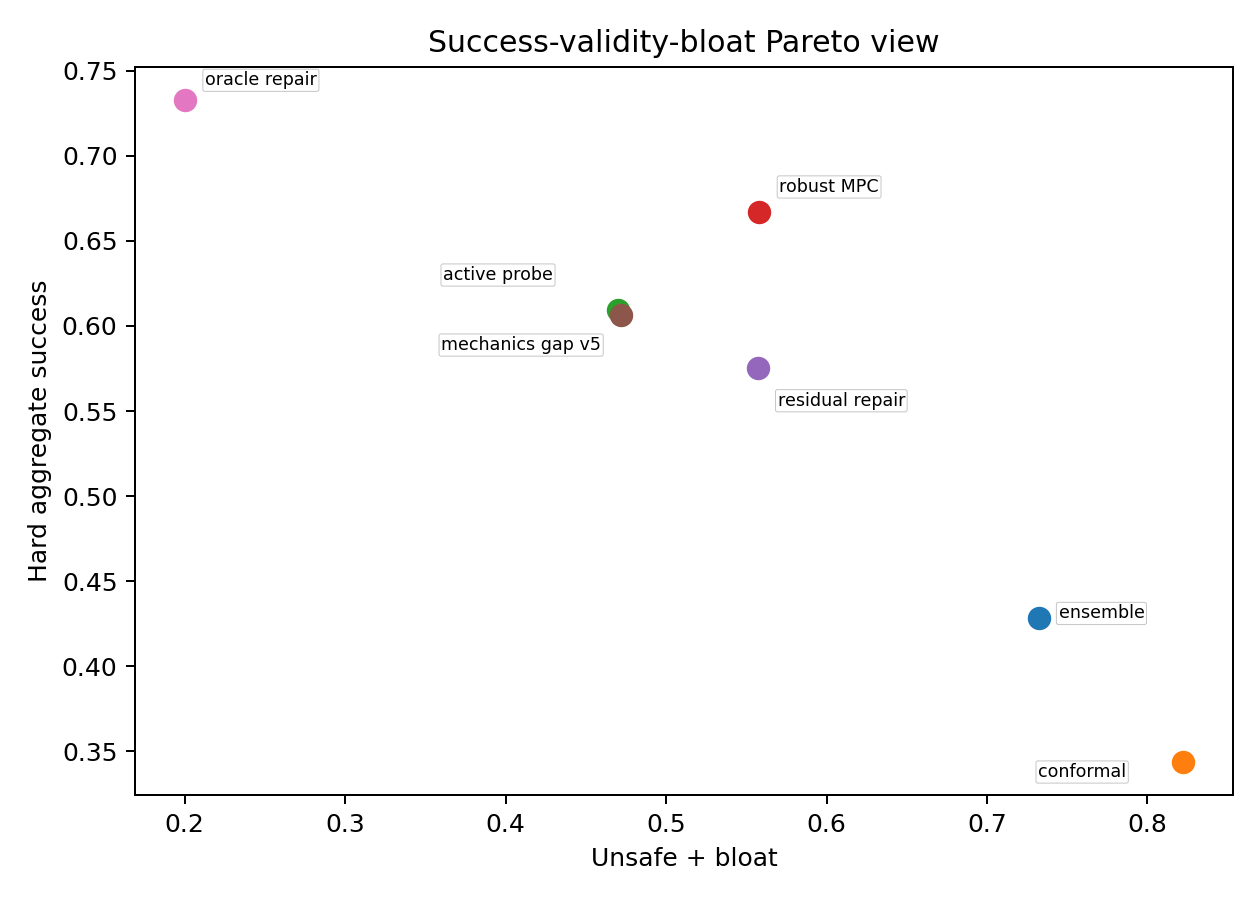
\includegraphics[width=0.9\linewidth]{uncertainty_bloat_pareto_v5.png}\caption{Hard-aggregate Pareto view for success, unsafe action, bloat, and utility.}\end{figure}

\section{Appendix: Raw Summary Extract}

\begin{center}
\scriptsize
\begin{longtable}{rp{0.84\linewidth}}
\caption{Wrapped extract from results/summary.txt.}\label{tab:summaryextract}\\
\toprule
Line & Summary extract\\
\midrule
\endfirsthead
\caption[]{Wrapped extract from results/summary.txt. (continued)}\\
\toprule
Line & Summary extract\\
\midrule
\endhead
1 & Paper 88 world\_model\_uncertainty\_bloat v5 expanded audit\\
2 & Terminal recommendation: KILL\_ARCHIVE\\
3 & ICLR main ready: no\\
4 & Reason: expanded CPU-only world-model uncertainty-bloat audit adds stronger UQ, conformal, active-probe, robust-MPC, residual-repair, Bayesian-expansion, ablation, stress, and fixed-risk tests, but no real robot or accepted high-f\\
5 & Main rollout rows: 199680\\
6 & Dataset summary rows: 15360\\
7 & Main seed-metric rows: 1040\\
8 & Main metric rows: 1248\\
9 & Main pairwise rows: 672\\
10 & Hard aggregate seed rows: 130\\
11 & Hard aggregate metric rows: 156\\
12 & Hard aggregate pairwise rows: 84\\
13 & Ablation rollout rows: 33600\\
14 & Ablation seed rows: 200\\
15 & Ablation metric rows: 20\\
16 & Stress raw rows: 302400\\
17 & Stress seed rows: 2520\\
18 & Stress metric rows: 252\\
19 & Fixed-risk raw rows: 69120\\
20 & Fixed-risk seed rows: 480\\
21 & Fixed-risk metric rows: 48\\
22 & Fixed-risk pairwise rows: 200\\
23 & Negative cases: 24\\
25 & Frozen hard-aggregate gate:\\
26 & best\_success\_reference=robust\_mpc\_fallback\\
27 & best\_f1\_reference=active\_probe\_then\_plan\\
28 & safest\_reference=robust\_mpc\_fallback\\
29 & lowest\_abstain\_reference=robust\_mpc\_fallback\\
30 & lowest\_bloat\_reference=active\_probe\_then\_plan\\
31 & best\_utility\_reference=robust\_mpc\_fallback\\
32 & proposal\_success=0.60642\\
33 & best\_success=0.66701\\
34 & proposal\_f1=0.58903\\
35 & best\_f1=0.56956\\
36 & proposal\_unsafe=0.13768\\
37 & safest\_unsafe=0.04861\\
38 & proposal\_abstain=0.08003\\
39 & lowest\_abstain=0.04792\\
40 & proposal\_bloat=0.33433\\
41 & lowest\_bloat=0.31471\\
42 & proposal\_utility=0.23714\\
43 & best\_utility=0.39872\\
44 & paired\_success\_lower95=-0.07734\\
45 & paired\_unsafe\_upper95=0.10347\\
46 & main\_gate=False\\
47 & mechanism\_gate=False\\
48 & stress\_gate=True\\
49 & stress\_dominated\_by=none\\
50 & fixed\_risk\_gate=False\\
51 & scope\_gate=False\\
52 & missing\_contact\_mode\_shift: v5\_coverage=0.00000, best\_feasible\_coverage=0.00000, v5\_success=0.00000, best\_feasible\_success=0.00000, v5\_unsafe=0.00000, best\_feasible\_unsafe=1.00000 | combined\_missing\_mechanics: v5\_coverage=0.00000,\\
54 & Hard aggregate metrics:\\
55 & mean\_world\_model\_mpc task\_success=0.51059 ci95=0.01382 f1=0.12245 unsafe=0.19149 false\_abstention=0.05747 bloat=0.32166 utility=0.08450\\
56 & ensemble\_variance\_gate task\_success=0.42812 ci95=0.00990 f1=0.40517 unsafe=0.13733 false\_abstention=0.24114 bloat=0.59478 utility=-0.14106\\
57 & mc\_dropout\_uncertainty task\_success=0.42899 ci95=0.01726 f1=0.38909 unsafe=0.12344 false\_abstention=0.23976 bloat=0.68705 utility=-0.14940\\
58 & conformal\_risk\_gate task\_success=0.34375 ci95=0.00998 f1=0.24982 unsafe=0.05747 false\_abstention=0.43906 bloat=0.76475 utility=-0.31438\\
59 & epistemic\_ensemble\_planner task\_success=0.52326 ci95=0.00701 f1=0.44923 unsafe=0.13472 false\_abstention=0.13246 bloat=0.51932 utility=0.06403\\
60 & active\_probe\_then\_plan task\_success=0.60938 ci95=0.01263 f1=0.56956 unsafe=0.15538 false\_abstention=0.04861 bloat=0.31471 utility=0.24197\\
61 & robust\_mpc\_fallback task\_success=0.66701 ci95=0.01149 f1=0.14463 unsafe=0.04861 false\_abstention=0.04792 bloat=0.50950 utility=0.39872\\
62 & residual\_dynamics\_repair task\_success=0.57517 ci95=0.01287 f1=0.48802 unsafe=0.15295 false\_abstention=0.07309 bloat=0.40408 utility=0.16994\\
63 & bayesian\_model\_expansion task\_success=0.56111 ci95=0.01820 f1=0.54754 unsafe=0.13195 false\_abstention=0.11389 bloat=0.41771 utility=0.15082\\
64 & uncertainty\_bloat\_audit\_v4 task\_success=0.54080 ci95=0.01434 f1=0.44907 unsafe=0.16701 false\_abstention=0.07413 bloat=0.51113 utility=0.08311\\
65 & mechanics\_gap\_auditor\_v5 task\_success=0.60642 ci95=0.01538 f1=0.58903 unsafe=0.13768 false\_abstention=0.08003 bloat=0.33433 utility=0.23714\\
66 & oracle\_mechanics\_repair task\_success=0.73264 ci95=0.00892 f1=0.72633 unsafe=0.08524 false\_abstention=0.04445 bloat=0.11493 utility=0.52000\\
67 & oracle\_full\_state\_policy task\_success=0.75851 ci95=0.00925 f1=0.75703 unsafe=0.05799 false\_abstention=0.04809 bloat=0.06241 utility=0.59694\\
69 & Key paired hard-aggregate differences:\\
70 & v5\_minus\_robust\_mpc\_fallback task\_success: mean=-0.06059 ci95=0.01675 lower95=-0.07734 upper95=-0.04384\\
71 & v5\_minus\_robust\_mpc\_fallback hidden\_mechanism\_f1: mean=0.44440 ci95=0.02174 lower95=0.42267 upper95=0.46614\\
72 & v5\_minus\_robust\_mpc\_fallback unsafe\_action: mean=0.08906 ci95=0.01440 lower95=0.07466 upper95=0.10347\\
73 & v5\_minus\_robust\_mpc\_fallback bloat\_index: mean=-0.17517 ci95=0.00202 lower95=-0.17719 upper95=-0.17315\\
74 & v5\_minus\_robust\_mpc\_fallback robust\_utility: mean=-0.16158 ci95=0.03182 lower95=-0.19340 upper95=-0.12976\\
75 & v5\_minus\_active\_probe\_then\_plan task\_success: mean=-0.00295 ci95=0.01759 lower95=-0.02054 upper95=0.01463\\
76 & v5\_minus\_active\_probe\_then\_plan hidden\_mechanism\_f1: mean=0.01947 ci95=0.02300 lower95=-0.00353 upper95=0.04247\\
77 & v5\_minus\_active\_probe\_then\_plan unsafe\_action: mean=-0.01771 ci95=0.01567 lower95=-0.03338 upper95=-0.00203\\
78 & v5\_minus\_active\_probe\_then\_plan bloat\_index: mean=0.01962 ci95=0.00246 lower95=0.01716 upper95=0.02209\\
79 & v5\_minus\_active\_probe\_then\_plan robust\_utility: mean=-0.00483 ci95=0.03990 lower95=-0.04473 upper95=0.03507\\
80 & v5\_minus\_robust\_mpc\_fallback task\_success: mean=-0.06059 ci95=0.01675 lower95=-0.07734 upper95=-0.04384\\
81 & v5\_minus\_robust\_mpc\_fallback hidden\_mechanism\_f1: mean=0.44440 ci95=0.02174 lower95=0.42267 upper95=0.46614\\
82 & v5\_minus\_robust\_mpc\_fallback unsafe\_action: mean=0.08906 ci95=0.01440 lower95=0.07466 upper95=0.10347\\
83 & v5\_minus\_robust\_mpc\_fallback bloat\_index: mean=-0.17517 ci95=0.00202 lower95=-0.17719 upper95=-0.17315\\
84 & v5\_minus\_robust\_mpc\_fallback robust\_utility: mean=-0.16158 ci95=0.03182 lower95=-0.19340 upper95=-0.12976\\
85 & v5\_minus\_uncertainty\_bloat\_audit\_v4 task\_success: mean=0.06562 ci95=0.02270 lower95=0.04292 upper95=0.08833\\
86 & v5\_minus\_uncertainty\_bloat\_audit\_v4 hidden\_mechanism\_f1: mean=0.13996 ci95=0.01933 lower95=0.12063 upper95=0.15929\\
87 & v5\_minus\_uncertainty\_bloat\_audit\_v4 unsafe\_action: mean=-0.02934 ci95=0.01703 lower95=-0.04637 upper95=-0.01231\\
88 & v5\_minus\_uncertainty\_bloat\_audit\_v4 bloat\_index: mean=-0.17680 ci95=0.00233 lower95=-0.17913 upper95=-0.17448\\
89 & v5\_minus\_uncertainty\_bloat\_audit\_v4 robust\_utility: mean=0.15403 ci95=0.04678 lower95=0.10725 upper95=0.20081\\
90 & v5\_minus\_robust\_mpc\_fallback task\_success: mean=-0.06059 ci95=0.01675 lower95=-0.07734 upper95=-0.04384\\
91 & v5\_minus\_robust\_mpc\_fallback hidden\_mechanism\_f1: mean=0.44440 ci95=0.02174 lower95=0.42267 upper95=0.46614\\
92 & v5\_minus\_robust\_mpc\_fallback unsafe\_action: mean=0.08906 ci95=0.01440 lower95=0.07466 upper95=0.10347\\
93 & v5\_minus\_robust\_mpc\_fallback bloat\_index: mean=-0.17517 ci95=0.00202 lower95=-0.17719 upper95=-0.17315\\
\bottomrule
\end{longtable}
\normalsize
\end{center}

\nocite{*}

\bibliographystyle{iclr2026_conference}

\bibliography{references}

\end{document}